% \iffalse
% This file builds on the class file `book.cls' to provide a thesis,
% minithesis, progress, project and report format, and on the class file `article.cls'
% to provide an article format, for use within the Dept. of Electronics
% and Computer Science at the University of Southampton.
%
% The thesis, minithesis, progress, project, report, gdp, gdpsummary and article environments are written to separate
% class files uosthesis.cls, uosminithesis.cls, uosprogress.cls, uosproject.cls, uosreport.cls, uosgdp.cls, uosgdpsummary.cls and uosarticle.cls.
% Copyright (C) 2001 by Steve R. Gunn
% Later Modifications (C) 2018 by Edward Longman
% Later Modifications (C) 2020 by Edward Longman
%    \begin{macrocode}
%<thesis|minithesis|progress|project|article|report|gdp|gdpsummary>\NeedsTeXFormat{LaTeX2e}[2007/02/26]
%    \end{macrocode}
%
%    Announce the document class and its version.
%
%    \begin{macrocode}
%<thesis>\ProvidesClass{uosthesis}
%<minithesis>\ProvidesClass{uosminithesis}
%<progress>\ProvidesClass{uosprogress}
%<project>\ProvidesClass{uosproject}
%<article>\ProvidesClass{uosarticle}
%<report>\ProvidesClass{uosreport}
%<gdp>\ProvidesClass{uosgdp}
%<gdpsummary>\ProvidesClass{uosgdpsummary}
%<*driver>
\ProvidesFile{uosdocs.drv}
%</driver>
%<*thesis|minithesis|progress|project|report|article|gdp|gdpsummary|driver>
              [2022/08/15 v1.6
%</thesis|minithesis|progress|project|report|article|gdp|gdpsummary|driver>
%<thesis|minithesis|progress|project|report|article|gdp|gdpsummary>   LaTeX document class]
%    \end{macrocode}
%
%    This bit of code contains the documentation driver file for
%    \TeX{}, i.e., the file that will produce the documentation you
%    are currently reading. It can be extracted from this file by the
%    {\sc docstrip} program.
%    \begin{macrocode}
%<*driver>
]
\documentclass[a4paper,10pt]{ltxdoc}
\GetFileInfo{uosdocs.drv} \CodelineIndex \EnableCrossrefs
%\RecordChanges
\setcounter{IndexColumns}{2}
\begin{document}
\DocInput{uosdocs.dtx}
\PrintIndex
%\PrintChanges
\end{document}
%</driver>
%    \end{macrocode}
% \fi
%
% \title{\LaTeXe{} Document Styles for the\\
%        University of Southampton\\
%       {File version \fileversion, dated \filedate}}
%
% \author{Edward Longman with prior work by Steve R. Gunn}
%
% \date{Printed \today}
%
% \maketitle
% \section{Quickstart}
%   This guide assumes you have installed MiKTeX or TeX live distributions.
%   It also requires having the program ``make'' for producing the templates again.
%
%   The folder labelled tex-mf should be installed in your local tex files
%   source or whatever your tex distro uses.
%
%   The Templates have been built for the Deparment of Electronics and Computer
%   Science in the Faculty of Engineering and Physical Science at the University
%   of Southampton.
%
%   The basic settings for University, Faculty and School are explained in Section~\ref{IntNames}
%
%   If a user only wishes to change the file for their thesis it is probably
%   easier to navigate to the class file labeled uosthesis and change the
%   department and faculty naming there. This will be located in the
%   subdirectory where you unzipped the files under tex/latex/uosdocs/
%
% \section{Description}
%
%    These \LaTeXe{} document classes are designed to produce thesis, mini-thesis, progress,
%    project, report, GDP report and GDP summary report documents which conformed to the
%    University of Southampton guidelines of April 2001. They were updated in Jan 2019 to
%    conform to changes in those guidelines. Specifically copyright and authorship
%    declaration changes. They are based on the document
%    class \texttt{book}, but modify some of its layout decisions. An article class is also
%    provided which is based on the document class \texttt{article}.
%
% \StopEventually{}
%
% \section{The {\sc docstrip} modules}
%
% The following modules are used in the implementation to direct
% {\sc docstrip} when generating the external files:
% \begin{center}
% \begin{tabular}{ll}
%   thesis            & produce the \texttt{uosthesis} document class\\
%   minithesis        & produce the \texttt{uosminithesis} document class\\
%   progress          & produce the \texttt{uosprogress} document class\\
%   project           & produce the \texttt{uosproject} document class\\
%   report            & produce the \texttt{uosreport} document class\\
%   article           & produce the \texttt{uosarticle} document class\\
%   gdp               & produce the \texttt{uosgdp} document class\\
%   gdpsummary        & produce the \texttt{uosgdpsummary} document class\\
%   testthesis        & produce an example thesis\\
%   testminithesis    & produce an example minithesis\\
%   testprogress      & produce an example progress\\
%   testproject       & produce an example project\\
%   testreport        & produce an example report\\
%   testarticle       & produce an example article\\
%   testgdp           & produce an example GDP report\\
%   testgdpsummary    & produce an example GDP summary report\\
%   introduction      & produce an example introduction chapter\\
%   conclusions       & produce an example conclusions chapter\\
%   appendix          & produce an example appendix chapter\\
%   figure            & produce an example figure file\\
%   definitions       & produce an example definitions file\\
%   references        & produce an example references file\\
%   bst               & produce a bibliography style file\\
%   driver            & produce a documentation driver file \\
% \end{tabular}
% \end{center}
%
% \section{Implementation}
%
% The checksum is to determine if there has been a truncation in the file during transmission over a network
%
%    The class has a custom option to define what colours should be used for links.
%    This option defines \texttt{sotoncolour} to use UoS palette colours.
%    Colour Code taken from \texttt{http://edshare.soton.ac.uk/10481}
%
%    All options are passed on to the \texttt{book} or \texttt{article} class.
%
%    \begin{macrocode}
%<*thesis|minithesis|progress|project|report|article|gdp|gdpsummary>
%    \end{macrocode}
%
% \begin{macro}{\baseclass}
%    \begin{macrocode}
%% ------------ Class/Formating Adjustment ----------------------
%% Adjust the book class to match the requirements
%% Set spacing, line and paragraph options
%% Set LaTeX builder options (work break penalties etc.)
%<*thesis|minithesis|progress|project|report|gdp|gdpsummary>
\def\baseclass{book}
%</thesis|minithesis|progress|project|report|gdp|gdpsummary>
%<*article>
\def\baseclass{article}
%</article>
%    \end{macrocode}
% \end{macro}
%
%    \begin{macrocode}
\RequirePackage{xcolor}
\colorlet{linkBlue}{blue}
\colorlet{custGray}{gray}
\colorlet{chapRed}{red}
\DeclareOption{sotoncolour}{
\definecolor{sotonMarineBlue}{RGB}{1,67,89} % Soton marine blue (P 7469C)
  \definecolor{sotonGrey}{RGB}{153,153,166} % Soton grey (P 443C)
  \definecolor{sotonRed}{RGB}{171,18,16} % Soton Red (P 484C)
  \colorlet{linkBlue}{sotonMarineBlue}
  \colorlet{custGray}{sotonGrey}
  \colorlet{chapRed}{sotonRed}
}
\DeclareOption*{\PassOptionsToClass{\CurrentOption}{\baseclass}}
%    \end{macrocode}
%
% \begin{macro}{\@checkoptions}
%
%    Before we can process the options we must deal with a small
%    problem.  That is, we want to change the default options of
%    the \texttt{book} or \texttt{article} class to \texttt{a4paper} and \texttt{11pt} or \texttt{12pt} but the
%    macro |\ProcessOptions| used by the \texttt{book} or \texttt{article} class
%    processes the options in the order specified in the
%    file.  Because \texttt{a4paper} is the first of the paper
%    sizing options it will be overridden by any user defined
%    option.  But the same is not true of the font size option
%    \texttt{11pt} or \texttt{12pt}.  To remedy this we define a macro
%    |\@checkoptions{|\meta{default}|}{|\meta{option-list}|}|
%    which checks to see if any options in \meta{option-list} have
%    been specified and if not adds \meta{default} to the option list.
%
%    \begin{macrocode}
\def\@checkoptions#1#2{
  \edef\@curroptions{\@ptionlist{\@currname.\@currext}}
  \@tempswafalse
  \@tfor\@this:=#2\do{
    \@expandtwoargs\in@{,\@this,}{,\@curroptions,}
    \ifin@ \@tempswatrue \@break@tfor \fi}
  \let\@this\@empty
  \if@tempswa \else \PassOptionsToClass{#1}{\baseclass}\fi
}
%    \end{macrocode}
% \end{macro}
%
%    With this macro at our disposal we can continue to
%    process the options
%
%    \begin{macrocode}
%<*thesis|minithesis|progress|report|article|gdp|gdpsummary>
\@checkoptions{11pt}{{10pt}{11pt}{12pt}}
%</thesis|minithesis|progress|report|article|gdp|gdpsummary>
%<*project>
\@checkoptions{12pt}{{10pt}{11pt}{12pt}}
%</project>
\PassOptionsToClass{a4paper}{\baseclass}
\ProcessOptions\relax
%    \end{macrocode}
%
%    and load the \texttt{book} or \texttt{article} document class
%    with A4 as the default paper size.
%
%    \begin{macrocode}
\LoadClass{\baseclass}
%    \end{macrocode}
%
% \subsection{Banner}
%
% \begin{macro}{\bhrule}
% \begin{macro}{\btypeout}
%
%    Provide a function to produce a banner on the output making the location
%    of the current section simpler.
%
%    \begin{macrocode}
\newcommand\bhrule{\typeout{------------------------------------------------------------------------------}}
\newcommand\btypeout[1]{\bhrule\typeout{\space #1}\bhrule}
%    \end{macrocode}
% \end{macro}
% \end{macro}
%
% \subsection{Date}
%
% \begin{macro}{\today}
%
%    This macro uses the \TeX\ primitives |\month|, |\day| and |\year|
%    to provide the date of the \LaTeX-run in a suitable format.
%
%    \begin{macrocode}
%<*thesis>
\def\today{\ifcase\month\or
  January\or February\or March\or April\or May\or June\or
  July\or August\or September\or October\or November\or December\fi
  \space \number\year}
%</thesis>
%    \end{macrocode}
%
% \end{macro}
%
% \section{Document Layout}
%
% \subsection{Font}
%    \begin{macrocode}
%% \usepackage[T1]{fontspec}
%    Set font for copyright statement body text
\usepackage[defaultsans]{droidsans}
%    Set a particular style of font for the thesis. A font that has smallcaps
\usepackage{mathpazo}
%%\usepackage[T1]{fontenc} %This may not be necessary for english only text
%    \end{macrocode}

% \subsection{Spacing}
%
%    Load the \texttt{setspace} package so that spacing can easily be set. The text in all
%    three styles is set to one and a half spacing, paragraphs not indented, and a newline
%    between paragraphs.
%
%    \begin{macrocode}
\usepackage{setspace}
%<thesis|minithesis|progress|project|report|gdp|gdpsummary>\onehalfspacing
%<article>\singlespacing
\setlength{\parindent}{0pt}
\setlength{\parskip}{2.0ex plus0.5ex minus0.2ex}
%    \end{macrocode}
%
%  \subsection{Margins}
%
%    Load the \texttt{geometry} package to setup the page dimensions.
%
%    \begin{macrocode}
\usepackage{geometry}
%<*thesis|minithesis|progress|project|report|gdp|gdpsummary>
\geometry{a4paper,
            % left=1.25in,
            % right=1.25in,
            hmarginratio=1:2,
            textwidth=146.5mm,
            top=0.6in,
            bottom=0.8in,
            headheight=20pt,
            headsep=0.25in,
            foot=9pt,
            footskip=0.3in,
            bindingoffset=0.5in,
            includeheadfoot}
%</thesis|minithesis|progress|project|report|gdp|gdpsummary>
%<*article>
\geometry{a4paper,
            % left=1.25in,
            % right=1.25in,
            hmarginratio=1:1,
            textwidth=169.4mm,
            top=0.6in,
            bottom=0.8in,
            headheight=20pt,
            headsep=0.25in,
            foot=9pt,
            footskip=0.3in,
            bindingoffset=0.5in,
            includeheadfoot}
%</article>
%    \end{macrocode}
%
% \subsection{Breaks}
%
%    Control how pages and lines are broken.
%
%    \begin{macrocode}
\raggedbottom
\setlength{\topskip}{1\topskip \@plus 5\p@}
\doublehyphendemerits=10000       % No consecutive line hyphens.
\brokenpenalty=10000              % No broken words across columns/pages.
\widowpenalty=9999                % Almost no widows at bottom of page.
\clubpenalty=9999                 % Almost no orphans at top of page.
\interfootnotelinepenalty=9999    % Almost never break footnotes.
%    \end{macrocode}
%
%  \subsection{Fancy Page Headers}
%
%    Setup the the default fancy page headers with an underlined header containing
%    chapter, name and page number.
%
%    \begin{macrocode}
\usepackage{fancyhdr}
% Help from https://texblog.org/2007/11/07/headerfooter-in-latex-with-fancyhdr/#comment-4783
\fancyhead[LE]{\textrm\thepage}
\fancyhead[LO]{\fancyplain{}{\textsl{\rightmark}}}
\fancyhead[RE]{\fancyplain{}{\textsl{\leftmark}}}
\fancyhead[RO]{\textrm\thepage}
\chead{}\lfoot{}\rfoot{}\cfoot{}
\pagestyle{fancy}
\fancypagestyle{plain}{
  \fancyhf{}
  \fancyhead[OR]{\thepage}
  \renewcommand{\headrulewidth}{0pt}
}
%    \end{macrocode}
%
% \begin{macro}{\chaptermark}
% \begin{macro}{\sectionmark}
% \begin{macro}{\subsectionmark}
%
%    Redefine \texttt{chaptermark} and \texttt{sectionmark} to set up the correct header name and produce a
%    banner on the output making the location of messages simpler.
%
% The \textbackslash btypeout command is for console logging where chapters start
%
% \textbackslash chapapp expands to "Chapter" or "Appendix"
%
%    \begin{macrocode}
%<*thesis|minithesis|progress|project|report|gdp>
\renewcommand{\chaptermark}[1]{\btypeout{\thechapter.\space #1}\markboth{\chaptername\ \thechapter.\hspace{1em}#1}{}}
\renewcommand{\sectionmark}[1]{\markright{\thesection.\hspace{1em}#1}}
\renewcommand{\subsectionmark}[1]{}
%</thesis|minithesis|progress|project|report|gdp>
%<*article>
\renewcommand{\sectionmark}[1]{\btypeout{\thesection\hspace{1em}}\markboth{}{\thesection.\hspace{1em}#1}}
\renewcommand{\subsectionmark}[1]{}
\renewcommand{\subsubsectionmark}[1]{}
%</article>
%<gdpsummary>\markboth{GDP Summary Report}{GDP Summary Report}
%    \end{macrocode}
% \end{macro}
% \end{macro}
% \end{macro}
%
% \begin{macro}{\cleardoublepage}
%
%    Redefine \texttt{cleardoublepage} to remove headers from blank pages
%    in twosided documents.
%
%    \begin{macrocode}
\def\cleardoublepage{\clearpage\if@twoside \ifodd\c@page\else
\hbox{}
\thispagestyle{empty}
\newpage
\if@twocolumn\hbox{}\newpage\fi\fi\fi}
%    \end{macrocode}
% \end{macro}
% \begin{macro}{\cleartoeven}
%
%    Define \texttt{cleartoeven} to remove headers from blank pages
%    and force to even page for appendix or index.
%
%    \begin{macrocode}
\def\cleartoeven{\clearpage\if@twoside \ifodd\c@page
\hbox{}
\thispagestyle{empty}
\newpage
\if@twocolumn\hbox{}\newpage\fi\fi\fi}
%    \end{macrocode}
% \end{macro}
%
% \subsection{Mathematics}
%
%    Load the \texttt{amsmath} packages, so we can do some serious math, and
%    setup the theorem environments.
%
%    \begin{macrocode}
%% -------------------- Figure/Table/Eq/Listing Stying --------------------
%% Set the styling for non text elements of the document
\usepackage{amsmath,amsfonts,amssymb,amscd,amsthm,xspace}
\theoremstyle{plain}
%<*thesis|minithesis|progress|project|report|gdp>
\newtheorem{example}{Example}[chapter]
\newtheorem{theorem}{Theorem}[chapter]
%</thesis|minithesis|progress|project|report|gdp>
%<*article|gdpsummary>
\newtheorem{example}{Example}[section]
\newtheorem{theorem}{Theorem}[section]
%</article|gdpsummary>
\newtheorem{corollary}[theorem]{Corollary}
\newtheorem{lemma}[theorem]{Lemma}
\newtheorem{proposition}[theorem]{Proposition}
\newtheorem{axiom}[theorem]{Axiom}
\theoremstyle{definition}
\newtheorem{definition}[theorem]{Definition}
\theoremstyle{remark}
\newtheorem{remark}[theorem]{Remark}
%    \end{macrocode}
%
% \subsection{Captions}
%
% \begin{macro}{\fref}
% \begin{macro}{\tref}
% \begin{macro}{\eref}
% \begin{macro}{\cref}
% \begin{macro}{\sref}
% \begin{macro}{\aref}
%
%   Load the \texttt{caption} package to improve formatting of captions,
%   and provide short referencing commands.
%
%    \begin{macrocode}
\usepackage[justification=centerlast,font=small,labelfont=sc]{caption}
\setlength{\captionmargin}{20pt}
\newcommand{\fref}[1]{Figure~\ref{#1}}
\newcommand{\tref}[1]{Table~\ref{#1}}
\newcommand{\eref}[1]{Equation~\ref{#1}}
\newcommand{\cref}[1]{Chapter~\ref{#1}}
\newcommand{\sref}[1]{Section~\ref{#1}}
\newcommand{\aref}[1]{Appendix~\ref{#1}}
%    \end{macrocode}
%
% \end{macro}
% \end{macro}
% \end{macro}
% \end{macro}
% \end{macro}
% \end{macro}
%
% \subsection{Float Placement}
%
% \begin{macro}{\topfraction}
% \begin{macro}{\textfraction}
%    Preventing figures from appearing on a page by themselves. \LaTeX's figure
%    placement algorithm is quite biased in favour of putting figures on a page
%    by themselves, instead of on the top of a page with some text below it.
%    Fortunately, the parameters of the algorithm can be changed. The main problem
%    is that \LaTeX\ per default only allows a part of the top of a text-page (70\%)
%    to contain figures, and requires at least 20\% of a page to be text when text and
%    figures share a page. These parameters should be set to more reasonable values,
%    for example 85\% and 10\%.
%    \begin{macrocode}
\renewcommand{\topfraction}{0.85}
\renewcommand{\bottomfraction}{.85}
\renewcommand{\textfraction}{0.1}
\renewcommand{\dbltopfraction}{.85}
%    \end{macrocode}
% \end{macro}
% \end{macro}
% \begin{macro}{\floatpagefraction}
%    This helps, but sometimes \LaTeX\ puts a figure on a page by itself, although it
%    would fit perfectly well on the top of a page. This happens when the figure will
%    not fit on the page where it was defined. \LaTeX\ then attempts to put it on a
%    figures-only page before it attempts to put it at the top of the next page. A page
%    may contain figures alone if the figure(s) use at least half the page. To prevent
%    half-empty pages this limit should probably be increased to around 75\%.
%    \begin{macrocode}
\renewcommand{\floatpagefraction}{0.75}
\renewcommand{\dblfloatpagefraction}{.75}
%    \end{macrocode}
%    Be careful not to make \texttt{floatpagefraction} larger than \texttt{topfraction},
%    then you risk to produce a figure that can neither go on the top of a text page,
%    nor on a page by itself. If that happens, the figure and all later figures will be
%    postponed until next time a \texttt{clearpage} is executed (typically at the end of
%    a chapter or the end of the document). This will also happen if a figure is too
%    large to fit on a page.
%    \begin{macrocode}
\setcounter{topnumber}{9}
\setcounter{bottomnumber}{9}
\setcounter{totalnumber}{20}
\setcounter{dbltopnumber}{9}
%    \end{macrocode}
% \end{macro}
%
%
% \subsection{Graphics}
%
%    Load the \texttt{graphicx} package, so we can include pictures easily. Load the \texttt{epstopdf},
%    so that eps files are automatically converted to pdf when pdf\LaTeX\ is used. This requires a
%   version of {\em epstopdf} to be installed on you system. You can find a windows version at\newline
%   \texttt{http://www.ctan.org/tex-archive/support/epstopdf/epstopdf.exe}.
%
%    \begin{macrocode}
\usepackage{graphicx}
\usepackage{epstopdf}
%    \end{macrocode}
%
% \subsection{Subfigures and subtables}
%
%    Load the \texttt{subcaption} package, so we can include subfigures easily.
%
%    \begin{macrocode}
\usepackage[]{subcaption}
\usepackage{booktabs}
\usepackage{rotating}
%    \end{macrocode}
%
% \subsection{Listings}
%
%    Load the \texttt{listings} package, so we can include listings easily.
%
%    \begin{macrocode}
\usepackage{listings}
% %\usepackage{lstpatch}
\lstset{captionpos=b,
        frame=tb,
        basicstyle=\scriptsize\ttfamily,
        showstringspaces=false,
        keepspaces=true}
\lstdefinestyle{matlab} {
        language=Matlab,
        keywordstyle=\color{blue},
        commentstyle=\color[rgb]{0.13,0.55,0.13}\em,
        stringstyle=\color[rgb]{0.7,0,0} }
%    \end{macrocode}
%
% \subsection{Hyperlinks}
%
%    Load the \texttt{hyperref} package to provide hyperlinks in pdf and dvi documents.
%
%    \begin{macrocode}
\usepackage[pdfpagemode={UseOutlines},bookmarks=true,bookmarksopen=true,
   bookmarksopenlevel=0,bookmarksnumbered=true,plainpages=false,pdfpagelabels,
   colorlinks,linkcolor={linkBlue},citecolor={linkBlue},urlcolor={linkBlue},
   pdfstartview={FitV},unicode,breaklinks=true]{hyperref}
\pdfstringdefDisableCommands{
   \let\\\space
}
%    \end{macrocode}
%
% \section{Internal Names}\label{IntNames}
%
% \begin{macro}{\supervisor}
% \begin{macro}{\examiner}
% \begin{macro}{\degree}
% \begin{macro}{\authors}
% \begin{macro}{\addresses}
% \begin{macro}{\university}
% \begin{macro}{\UNIVERSITY}
% \begin{macro}{\department}
% \begin{macro}{\DEPARTMENT}
% \begin{macro}{\group}
% \begin{macro}{\GROUP}
% \begin{macro}{\faculty}
% \begin{macro}{\FACULTY}
% \begin{macro}{\subject}
% \begin{macro}{\keywords}
%
%    The various elements of the documents are defined
%    as control sequences to make it easy to customize this
%    style for other parts of the University. When the
%    command is run the other terms are defined by the args.
%
%    The examiner and supervisor commands can be puralised
%    so that it can print "Supervisors:". This is with an
%    optional argument. [s] which will add and ``s'' to the
%    word "Supervisor"
%
%    \begin{macrocode}
%% --------------------- Organisational Structure ----------------------
\newcommand*{\supervisor}[2][]{\def\supname{#2}\def\supplural{#1}}
\newcommand*{\examiner}[2][]{\def\examname{#2}\def\examplural{#1}}
\newcommand*{\degree}[1]{\def\degreename{#1}}
\newcommand*{\authors}[1]{\def\authornames{#1}}
\newcommand*{\qualifications}[1]{\def\quals{#1}}
\newcommand*{\addresses}[1]{\def\addressnames{#1}}
\newcommand*{\documentDoi}[1]{\def\doicode{#1}}
\newcommand*{\volume}[2]{\def\volno{#1}\def\volof{#2}}
\newcommand*{\orcidid}[1]{\def\orcid{#1}}
\newcommand*{\university}[1]{\def\univname{#1}}
\newcommand*{\UNIVERSITY}[1]{\def\UNIVNAME{#1}}
\newcommand*{\department}[1]{\def\deptname{#1}}
\newcommand*{\DEPARTMENT}[1]{\def\DEPTNAME{#1}}
\newcommand*{\group}[1]{\def\groupname{#1}}
\newcommand*{\GROUP}[1]{\def\GROUPNAME{#1}}
\newcommand*{\faculty}[1]{\def\facname{#1}}
\newcommand*{\FACULTY}[1]{\def\FACNAME{#1}}
\newcommand*{\subject}[1]{\def\subjectname{#1}}
\newcommand*{\keywords}[1]{\def\keywordnames{#1}}
%    \end{macrocode}
%
% \end{macro}
% \end{macro}
% \end{macro}
% \end{macro}
% \end{macro}
% \end{macro}
% \end{macro}
% \end{macro}
% \end{macro}
% \end{macro}
% \end{macro}
% \end{macro}
% \end{macro}
% \end{macro}
% \end{macro}
%
%
% \begin{macro}{\supname}
% \begin{macro}{\examname}
% \begin{macro}{\degreename}
% \begin{macro}{\authornames}
% \begin{macro}{\univname}
% \begin{macro}{\UNIVNAME}
% \begin{macro}{\deptname}
% \begin{macro}{\DEPTNAME}
% \begin{macro}{\groupname}
% \begin{macro}{\GROUPNAME}
% \begin{macro}{\facname}
% \begin{macro}{\FACNAME}
% \begin{macro}{\subjectname}
% \begin{macro}{\keywordnames}
%
%    The internal names of the elements are set
%    to defaults appropriate to the Department of Electronics and Computer Science.
%
%    By running these commands at the top of your tex file it will overwrite the defaults.
%    \begin{macrocode}
%% --------------------- Organisational Structure ----------------------
\documentDoi{}
\supervisor  {}
\examiner    {}
\degree      {}
\authors     {}
\qualifications{}
\orcidid{}
\volume{}{}
\university  {\texorpdfstring{\href{http://www.southampton.ac.uk}
                {University of Southampton}}
                {University of Southampton}}
\UNIVERSITY  {\MakeUppercase{\univname}}
\department  {School of Electronics and Computer Science}
\DEPARTMENT  {\MakeUppercase{\deptname}}
\group       {}
\GROUP       {\MakeUppercase{\groupname}}
\faculty     {Faculty of Engineering and Physical Science}
\FACULTY     {\MakeUppercase{\facname}}
\addresses   {}
\subject     {}
\keywords    {}
%    \end{macrocode}
%
% \end{macro}
% \end{macro}
% \end{macro}
% \end{macro}
% \end{macro}
% \end{macro}
% \end{macro}
% \end{macro}
% \end{macro}
% \end{macro}
% \end{macro}
% \end{macro}
% \end{macro}
% \end{macro}
%
% \section{Special Pages}
%
% \subsection{Title Page}
%
% \begin{macro}{\maketitle}
%
%    Setup an appropriate title page and pdf strings if we are using
%    pdf\LaTeX.
%
%    The %\\global\\let\\@title\\@empty has been removed
%
%    Possibly the relax statement also needs to be removed
%
%   \begin{macrocode}
%<*thesis|minithesis|progress|project|report|gdp|gdpsummary>}
%    Start by Adding meta data to the produced document
\usepackage{titling}
\AtBeginDocument{
  \hypersetup{pdftitle={\thetitle}}
  \hypersetup{pdfsubject={\subjectname}}
  \hypersetup{pdfauthor={\authornames}}
  \hypersetup{pdfkeywords={\keywordnames}}
}
%    Define the title page layout
\renewcommand\maketitle{
  \btypeout{Title Page}
  \thispagestyle{empty}
  \begin{titlepage}
    \let\footnotesize\small
    \let\footnoterule\relax
    \let \footnote \thanks
    \setcounter{footnote}{0}
    \null\vfil
    \vskip 60\p@
    \begin{center}
      \setlength{\parskip}{0pt}
      {\scshape\LARGE\textbf{\univname}\par}
      %% TODO: Change all the descriptions to italic like the Thesis one
%<*thesis|minithesis|progress|project|gdp|gdpsummary>
      \bigskip
      {\large \facname \par}
      {\large \deptname \par}
%</thesis|minithesis|progress|project|gdp|gdpsummary>
%<*thesis|minithesis|progress>
      {\large \groupname \par}
%</thesis|minithesis|progress>
      \vfill
%<*minithesis>
      {\large A mini-thesis submitted for transfer from}
      {\large MPhil to PhD \par}
%</minithesis>
%<*progress>
      {\large A progress report submitted for continuation}
      {\large towards a PhD \par}
%</progress>
%<*project>
      {\large A project report submitted for the}
      {\large award of \par \degreename \par}
%</project>
%<*gdp>
      {\large A group design project report submitted for}
      {\large the award of \par \degreename \par}
%</gdp>
%<*gdpsummary>
      {\large A group design project summary report submitted}
      {\large for the award of \par \degreename \par}
%</gdpsummary>
%<*minithesis|progress|project>
      \vfill
      {\normalsize Supervisor\supplural: \supname \par}
      \ifthenelse{\isempty{\examname}}
      {\normalsize Examiner\examplural: \examname \par}{}
      \vfill
      \hspace{6mm}\parbox[t][51mm][s]{89mm}{
        \center
        \vfill
        {\large \bf \@title \par}
        \vfill
        {\normalsize \textit{by} \textbf\authornames \par}
        \vfill
        {\normalsize \@date \par}
        \vfill
      }
      \parbox[t][95mm][s]{89mm}{}
%</minithesis|progress|project>
%<*gdp|gdpsummary>
      \vfill
      {\normalsize \textit{by} \textbf\authornames \par}
      \bigskip
      {\normalsize Supervisor\supplural: \supname \par}
      {\normalsize Examiner\examplural: \examname \par}
      \vfill
      \hspace{6mm}\parbox[t][51mm][s]{89mm}{
        \center
        \vfill
        {\large \bf \@title \par}
        \vfill
        {\normalsize \@date \par}
        \vfill
      }
      \parbox[t][95mm][s]{89mm}{}
%</gdp|gdpsummary>
%<*thesis|report>
      {\huge \bf \@title \par
}
      \ifthenelse{\equal{\doicode}{}}
      {}
      {\smallskip DOI: \href{https://doi.org/\doicode}{\doicode}\par}
      \ifthenelse{\equal{\volno}{}}
      {}
      {\smallskip Volume \volno{} of \volof}
      \vfill
      {\LARGE \textit{by} \par}
      \smallskip
      {\LARGE \textbf\authornames
        \ifthenelse{\equal{\quals}{}}
        {}
        {\par\Large
        \quals}
      \par}
        \ifthenelse{\equal{\orcid}{}}
        {}
        {\smallskip
        ORCID iD: \href{https://orcid.org/\orcid}{\orcid}}

      \vfill
%<*thesis>
      {\large \textit{A thesis for the degree of} \par}
      {\large \textit{Doctor of Philosophy} \par}
%</thesis>
%<*report>      {\large  \textit{Technical Report} \par}
      \bigskip
\bigskip
      {\large \facname \par}
      {\large \deptname \par}
%</report>
      \bigskip
      \bigskip
      \bigskip
      {\Large \@date \par}
      \bigskip
%</thesis|report>
    \end{center}
    \par
    \@thanks
    \vfil\null
  \end{titlepage}
  \setcounter{footnote}{0}%
  \global\let\thanks\relax
  \global\let\maketitle\relax
  \global\let\@thanks\@empty
  \global\let\@author\@empty
  \global\let\@date\@empty
  \global\let\title\relax
  \global\let\author\relax
  \global\let\date\relax
  \global\let\and\relax
%<*thesis|minithesis|progress|project|report>
  \cleardoublepage
%</thesis|minithesis|progress|project|report>
}
%</thesis|minithesis|progress|project|report|gdp|gdpsummary>
%<*article>
\if@titlepage
  \renewcommand\maketitle{
    \btypeout{Title Page}
    \markboth{\authornames}{\@title}
    \begin{titlepage}
    \thispagestyle{empty}
    \let\footnotesize\small
    \let\footnoterule\relax
    \let \footnote \thanks
    \null\vfil
    \vskip 60\p@
    \begin{center}
      {\LARGE \@title \par}
      \vskip 3em
      {\large \lineskip .75em
        \begin{tabular}[t]{c} \authornames \end{tabular}
      \par}
      \vskip 1em
      {\large \lineskip .5em
        \begin{tabular}[t]{c} \addressnames \end{tabular}
      \par}
      \vskip 1.5em
      {\large \@date \par}
      \if\keywordnames
      \else
        \quotation
        \vskip 1.5em
        {\noindent \normalsize
            \textbf{Keywords:}
            \textit{\keywordnames}
        \par}
        \endquotation
      \fi
    \end{center}
    \par
    \@thanks
    \vfil\null
    \end{titlepage}
    \setcounter{footnote}{0}
    \global\let\thanks\relax
    \global\let\maketitle\relax
    \global\let\@maketitle\relax
    \global\let\@thanks\@empty
    \global\let\@author\@empty
    \global\let\@date\@empty
    \global\let\title\relax
    \global\let\author\relax
    \global\let\date\relax
    \global\let\and\relax
  }
\else
  \renewcommand\maketitle{
    \btypeout{Title Page}
    \markboth{\authornames}{\@title}
    \thispagestyle{empty}
    \par
    \begingroup
      \renewcommand\thefootnote{\@fnsymbol\c@footnote}
      \def\@makefnmark{
        \rlap{\@textsuperscript{\normalfont\@thefnmark}}
      }
      \long\def\@makefntext##1{
        \parindent 1em\noindent \hb@xt@1.8em
        {\hss\@textsuperscript{\normalfont\@thefnmark}}##1
      }
      \if@twocolumn
        \ifnum \col@number=\@ne
          \@maketitle
        \else
          \twocolumn[\@maketitle]%
        \fi
      \else
        \newpage
        % Prevent figures from going at top of page.
        \global\@topnum\z@
        \@maketitle
      \fi
      \thispagestyle{plain}\@thanks
    \endgroup
    \setcounter{footnote}{0}%
    \global\let\thanks\relax
    \global\let\maketitle\relax
    \global\let\@maketitle\relax
    \global\let\@thanks\@empty
    \global\let\@author\@empty
    \global\let\@date\@empty
    \global\let\title\relax
    \global\let\author\relax
    \global\let\date\relax
    \global\let\and\relax
  }
  \def\@maketitle{
    \newpage
    \null
    \vskip 2em
    \begin{center}
      \let \footnote \thanks
      {\LARGE \@title \par}
      \vskip 1.5em
      {\large \lineskip .5em
        \begin{tabular}[t]{c} \authornames \end{tabular}
      \par}
      \vskip 0.7em
      {\large \lineskip .5em
        \begin{tabular}[t]{c} \addressnames \end{tabular}
      \par}
      \vskip 1em
      {\large \@date}
    \end{center}
    \par
    \vskip 1.5em
  }
\fi
%</article>
%    \end{macrocode}
%
% \end{macro}
%
% \subsection{Abstract Page}
%
% \begin{macro}{\abstract}
%
%    Setup an appropriate abstract page.
%
%    \begin{macrocode}
%<*thesis|minithesis|progress|project|report|gdp>
\newenvironment{abstract}
{
  \btypeout{Abstract Page}
  \thispagestyle{empty}
  \null\vfil\vfil
  \begingroup
   \centering
    \setlength{\parskip}{0pt}
    {\textsc\normalsize \univname \par}
    \bigskip
    {\underline{Abstract} \par}
%<*thesis|minithesis|progress|project|report>
    \bigskip
    {\textsc\normalsize \facname \par}
    {\textsc\normalsize \deptname \par}
%</thesis|minithesis|progress|project|report>
    \bigskip
%<*thesis>
    {\normalsize \underline{Doctor of Philosophy}\par}
%</thesis>
%<*minithesis>
    {\normalsize \underline{A mini-thesis submitted for transfer from MPhil to PhD}\par}
%</minithesis>
%<*progress>
    {\normalsize \underline{A progress report submitted for continuation towards a PhD}\par}
%</progress>
%<*project>
    {\normalsize \underline{A project report submitted for the award of \degreename}\par}
%</project>
    \bigskip
    {\normalsize\bf \@title \par}
    \medskip
    {\normalsize by \authornames \par}
    \bigskip
  \endgroup
}
{
%<*thesis|minithesis|progress|project|report>
  \vfil\vfil\null
  \cleardoublepage
%</thesis|minithesis|progress|project|report>
}
%</thesis|minithesis|progress|project|report|gdp>
%<*article>
\if@titlepage
  \renewenvironment{abstract}{
      \titlepage
      \null\vfil
      \@beginparpenalty\@lowpenalty
      \begin{center}
        \bfseries \abstractname
        \@endparpenalty\@M
      \end{center}
      \begin{itshape}
      \noindent
  }
  {
      \par
      \end{itshape}
      \if\keywordnames
      \else
        \quote
        \vskip 1.5em
        {\noindent \normalsize
            \textbf{Keywords:}
            \textit{\keywordnames}
        \par}
        \endquote
      \fi
      \vfil\null\endtitlepage
  }
\else
  \renewenvironment{abstract}{
      \if@twocolumn
        \section*{\abstractname}
      \else
        \small
        \begin{center}
          {\bfseries \abstractname\vspace{-.5em}\vspace{\z@}}
        \end{center}
        \quote
      \fi
      \begin{itshape}
  }
  {
      \end{itshape}
      \if\keywordnames
      \else
        \vskip 1.5em
        {\noindent \normalsize
            \textbf{Keywords:}
            \textit{\keywordnames}
        \par}
      \fi
      \if@twocolumn\else\endquote\fi
  }
\fi
%</article>
%    \end{macrocode}
%
% \end{macro}
%
% \subsection{Contents Pages}
% Possibly all of these pages should be redone by using the tocloft package to reduce
% complexity in this style file.
%
% \subsubsection{Add to Table of Contents}
%
% \begin{macro}{\addtotoc}
%    Get a better list of contents package
%
%    Ensures numbering for sub-subsections in the table of contents, and provide
%    for 6 levels to appear in toc. Define \texttt{addtotoc} to enable adding
%    elements to the toc at chapter level, using a dummy counter to fix bookmarks
%    in pdf\LaTeX{}.
%
%    \begin{macrocode}
%<*thesis|minithesis|progress|project|report|gdp|article>
\usepackage[nottoc]{tocbibind}         % Put the Lists, Glossary, Biblog and Idx in the contents
\addtocounter{secnumdepth}{1}
\setcounter{tocdepth}{6}
\newcounter{dummy}
\newcommand\addtotoc[1]{
\refstepcounter{dummy}
%<*thesis|minithesis|progress|project|report|gdp>
\addcontentsline{toc}{chapter}{#1}}
%</thesis|minithesis|progress|project|report|gdp>
%<*article>
\addcontentsline{toc}{section}{#1}}
%</article>
%    \end{macrocode}
% \end{macro}
% \subsubsection{Table of Contents}
%
% \begin{macro}{\tableofcontents}
%
%    Adjust line and paragraph spacing.
%
%    \begin{macrocode}
\renewcommand\tableofcontents{
\hypersetup{linkcolor={black}}
\btypeout{Table of Contents}
\begin{spacing}{1}{
    \setlength{\parskip}{1pt}
    \if@twocolumn
      \@restonecoltrue\onecolumn
    \else
      \@restonecolfalse
    \fi
%<*thesis|minithesis|progress|project|report|gdp>
    \chapter*{\contentsname
%</thesis|minithesis|progress|project|report|gdp>
%<*article>
    \section*{\contentsname
%</article>
        \@mkboth{
           \MakeUppercase\contentsname}{\MakeUppercase\contentsname}}
    \@starttoc{toc}
    \if@restonecol\twocolumn\fi
%<thesis|minithesis|progress|project|report|gdp>   \cleardoublepage
}\end{spacing}
}
%    \end{macrocode}
% \end{macro}
%
% \subsubsection{List of Figures}
%
% \begin{macro}{\listoffigures}
%
%    Adjust line and paragraph spacing.
%
%    \begin{macrocode}
\renewcommand\listoffigures{
\addtotoc{\listfigurename}
\begin{spacing}{1}{
    \setlength{\parskip}{1pt}
    \if@twocolumn
      \@restonecoltrue\onecolumn
    \else
      \@restonecolfalse
    \fi
%<*thesis|minithesis|progress|project|report|gdp>
    \chapter*{\listfigurename
%</thesis|minithesis|progress|project|report|gdp>
%<*article>
    \section*{\listfigurename
%</article>
      \@mkboth{\MakeUppercase\listfigurename}
              {\MakeUppercase\listfigurename}}
    \@starttoc{lof}
    \if@restonecol\twocolumn\fi
%<*thesis|minithesis|progress|project|report|gdp>
    \cleardoublepage
%</thesis|minithesis|progress|project|report|gdp>
}\end{spacing}
}
%    \end{macrocode}
% \end{macro}
%
% \subsubsection{List of Tables}
%
% \begin{macro}{\listoftables}
%
%    Adjust line and paragraph spacing.
%
%    \begin{macrocode}
\renewcommand\listoftables{
\addtotoc{\listtablename}
\begin{spacing}{1}{
    \setlength{\parskip}{1pt}
    \if@twocolumn
      \@restonecoltrue\onecolumn
    \else
      \@restonecolfalse
    \fi
%<*thesis|minithesis|progress|project|report|gdp>
    \chapter*{\listtablename
%</thesis|minithesis|progress|project|report|gdp>
%<*article>
    \section*{\listtablename
%</article>
      \@mkboth{
          \MakeUppercase\listtablename}{\MakeUppercase\listtablename}}
    \@starttoc{lot}
    \if@restonecol\twocolumn\fi
%<*thesis|minithesis|progress|project|report|gdp>
    \cleardoublepage
%</thesis|minithesis|progress|project|report|gdp>
}\end{spacing}
}
%    \end{macrocode}
% \end{macro}
%
% \subsubsection{List of Symbols}
%
% \begin{macro}{\listsymbolname}
% \begin{macro}{\listofsymbols}
%
%    Provide a \texttt{listofsymbols} command to produce a list of symbols,
%
%    \begin{macrocode}
%<*thesis|minithesis|progress|report|article>
\newcommand\listsymbolname{Definitions and Abbreviations}
%</thesis|minithesis|progress|report|article>
%<*project|gdp>
\newcommand\listsymbolname{List of Symbols}
%</project|gdp>
\usepackage{longtable}
\newcommand\listofsymbols[2]{
\btypeout{\listsymbolname}
\addtotoc{\listsymbolname}
%<*thesis|minithesis|progress|project|report|gdp>
    \chapter*{\listsymbolname
%</thesis|minithesis|progress|project|report|gdp>
%<*article>
    \section*{\listsymbolname
%</article>
      \@mkboth{
          \MakeUppercase\listsymbolname}{\MakeUppercase\listsymbolname}}
\begin{longtable}[c]{#1}#2\end{longtable}\par
%<*thesis|minithesis|progress|project|report|gdp>
    \cleardoublepage
%</thesis|minithesis|progress|project|report|gdp>
}
%</thesis|minithesis|progress|project|report|gdp|article>
%    \end{macrocode}
%
% \end{macro}
% \end{macro}
%
% \subsubsection{List of Additional Material}
%
% \begin{macro}{\addmaterialname}
% \begin{macro}{\listofaddmaterial}
% \begin{macro}{\addtolom}
%
%    Provide a \texttt{listofaddmaterial} command to produce a list of additional material,
%    the name can be changed with \verb|\addmaterialname{NewName}|
%
%    Material can be added by using \verb|\addcontentsline{lom}{chapter}{Material Name}|
%
%    \begin{macrocode}
\newcommand\addmaterialname{List of Additional Material}
\newcommand\listofaddmaterial{
\addtotoc{\addmaterialname}
\begin{spacing}{1}{
    \setlength{\parskip}{1pt}
    \if@twocolumn
      \@restonecoltrue\onecolumn
    \else
      \@restonecolfalse
    \fi
%<*thesis|minithesis|progress|project|report|gdp>
    \chapter*{\addmaterialname
%</thesis|minithesis|progress|project|report|gdp>
%<*article|gdpsummary>
    \section*{\addmaterialname
%</article|gdpsummary>
      \@mkboth{
          \MakeUppercase\addmaterialname}{\MakeUppercase\addmaterialname}}
    \@starttoc{lom}
    \if@restonecol\twocolumn\fi
%<*thesis|minithesis|progress|project|report|gdp>
    \cleardoublepage
%</thesis|minithesis|progress|project|report|gdp>
}\end{spacing}
}
\newcommand\addtolom[1]{%
\addtocontents{lom}{\protect\contentsline{chapter}{\protect\numberline{}#1}{}{}}
}
%    \end{macrocode}
%
% \end{macro}
% \end{macro}
% \end{macro}
%
% \subsection{Declaration of Authorship}
% \begin{macro}{\authorshipdeclaration}
% Taken from Modified Template by Lovell \ref{references}
%
% TODO: Consider a separate dissertation class for non techinical?
%
% TODO: Provide extra argument for putting the date into the Declaration
%
% This Authorship macro takes one argument for the case of People
% who have published part of their thesis already (perhaps in a paper).
%
% This authoship macro produces the statement of Originality for the gdp class.
% The authorship is normally done in custom appendix for projects like this.
%
% xifthen else package used for the isempty command
%
%    \begin{macrocode}
%<*thesis|minithesis|progress|report|article|project>
\usepackage{xifthen}
\newcommand\authorshipdeclaration[1]{
\btypeout{Declaration of Authorship}
\addtotoc{Declaration of Authorship}
\thispagestyle{plain}
\null\vfil
\vskip 60\p@
\begin{center}{\Large\bf Declaration of Authorship \par}\end{center}
I declare that this thesis and the work presented in it is my own and has
been generated by me as the result of my own original research.

I confirm that:

\begin{enumerate}
%<*thesis|minithesis|progress|article>
\item This work was done wholly or mainly while in candidature for a research degree at this University;
\item Where any part of this thesis has previously been submitted for a degree or any other qualification at this University or any other institution, this has been clearly stated;
%</thesis|minithesis|progress|article>
%<*project|report>
\item This work was done wholly or mainly while in candidature for a degree at this University;
\item Where any part of this report has previously been submitted for any other qualification at this University or any other institution, this has been clearly stated;
%</project|report>
\item Where I have consulted the published work of others, this is always clearly attributed;
\item Where I have quoted from the work of others, the source is always given. With the exception of such quotations, this thesis is entirely my own work;
\item I have acknowledged all main sources of help;
\item Where the thesis is based on work done by myself jointly with others, I have made clear exactly what was done by others and what I have contributed myself;

\ifthenelse{\isempty{#1}}
{\item None of this work has been published before submission}
{\item Parts of this work have been published as: #1}
\end{enumerate}

\vspace{15.0mm}
\begin{minipage}[t]{0.7\textwidth}
  Signed:..........................................................................
\end{minipage}%
\begin{minipage}[t]{0.3\textwidth}
  Date:..................
\end{minipage}
\vfil\vfil\null
\cleardoublepage
}
%</thesis|minithesis|progress|report|article|project>
%<*gdp>
\usepackage{xifthen}
\newcommand\authorshipdeclaration[2][]{
\btypeout{Declaration of Authorship}
\addtotoc{Statement of Originality}
\thispagestyle{plain}
\null\vfil
\vskip 60\p@
\begin{center}{\Large\bf Statement of Originality \par}\end{center}
%TODO Check Spelling

\begin{enumerate}

\ifthenelse{\isempty{#1}}
{
\item I have read and understood the ECS Academic Integrity information
%% http://ecs.gg/ai
and the University’s Academic Integrity Guidance for Students.
%% https://www.southampton.ac.uk/quality/assessment/academic_integrity.page
\item I am aware that failure to act in accordance with the Regulations Governing Academic Integrity
%% http://www.calendar.soton.ac.uk/sectionIV/academic-integrity-regs.html
may lead to the imposition of penalties which, for the most serious cases, may include termination of programme.
\item I consent to the University copying and distributing any or all of my work in any form and using third parties (who may be based outside the EU/EEA) to verify whether my work contains plagiarised material, and for quality assurance purposes.}
{#1}
%% The project specific statements
#2
\end{enumerate}
\vfil\vfil\null
\cleardoublepage
}
%</gdp>
%    \end{macrocode}
%
% \end{macro}
%
% \subsection{Copyright Statement}
% \begin{macro}{\copyrightDeclaration}
%
%    This standard Copyright statement is to be included for a thesis submission
%    to University of Southampton Digital Repository
%
%    \begin{macrocode}
%<*thesis>
\usepackage[export]{adjustbox} % for Soton logo alignment
\newcommand\copyrightDeclaration[1]{

\btypeout{Copyright declaration}
\thispagestyle{plain}

\hspace{-1.5in}\hspace{2.5cm}\begin{minipage}{17cm}
\null\vfil

\includegraphics[width=6cm,right]{UoSLogo.pdf}

\vskip 60\p@
\begin{center}{\selectfont\huge
\textcolor{custGray}{University~of~Southampton~Research~Repository}\par}
\end{center}
\vspace{1cm}

{\droidsans

\noindent Copyright \textcopyright{} and Moral Rights for this thesis and, where
applicable, any accompanying data are retained by the author and/or other
copyright owners. A copy can be downloaded for personal non-commercial research
or study, without prior permission or charge. This thesis and the accompanying
data cannot be reproduced or quoted extensively from without first obtaining
permission in writing from the copyright holder/s. The content of the thesis
and accompanying research data (where applicable) must not be changed in any
way or sold commercially in any format or medium without the formal permission
of the copyright holder/s.

\vspace{0.5cm}

When referring to this thesis and any accompanying data, full bibliographic
details must be given, e.g.

\vspace{0.5cm}

Thesis: Author (Year of Submission) ``Full thesis title'', University of
Southampton, name of the University Faculty or School or Department,
PhD Thesis, pagination.

\vspace{0.5cm}

Data: Author (Year) Title. URI [dataset]}
\end{minipage}
\vfil\vfil\null
\cleardoublepage
}

\usepackage{lastpage} % counts the full number of pages

%</thesis>
%    \end{macrocode}
%
% \end{macro}


% \subsection{Acknowledgements}
%
% \begin{macro}{\acknowledgements}
%
%    Thank someone!
%
%    \begin{macrocode}
\newcommand\acknowledgements[1]{
\btypeout{Acknowledgements}
\addtotoc{Acknowledgements}
%<*thesis|minithesis|progress|project|report|gdp>
\thispagestyle{plain}
\null\vfil
\vskip 60\p@
\begin{center}{\Large\bf Acknowledgements \par}\end{center}
{\normalsize #1}
\vfil\vfil\null
\cleardoublepage
%</thesis|minithesis|progress|project|report|gdp>
%<*article>
\section*{Acknowledgements}
{\normalsize #1}
%</article>
}
%    \end{macrocode}
%
% \end{macro}
%
% \subsection{Dedicatory}
%
% \begin{macro}{\dedicatory}
%
%    Dedicate the document to someone!
%
%    \begin{macrocode}
\newcommand\dedicatory[1]{
\btypeout{Dedicatory}
%<*thesis|minithesis|progress|project|report|gdp>
\thispagestyle{plain}
\null\vfil
\vskip 60\p@
\begin{center}{\Large \sl #1}\end{center}
\vfil\null
\cleardoublepage
%</thesis|minithesis|progress|project|report|gdp>
}
%    \end{macrocode}
%
% \end{macro}
%
% \section{Parts}
%
% \begin{macro}{\frontmatter}
% \begin{macro}{\mainmatter}
% \begin{macro}{\backmatter}
% \begin{macro}{\appendix}
%
%    Define \texttt{frontmatter},\texttt{mainmatter},\texttt{backmatter} for the article class
%    and rename the bibliography to something that makes more sense. For other classes make the
%    Appendix entry in the table of contents better and rename the references in a slightly
%    different way.
%
%    \begin{macrocode}
%<*article>
\newcommand\frontmatter{ }
\newcommand\mainmatter{ }
\newcommand\bibname{References}
\newcommand\backmatter{}
%</article>
%<*thesis|minithesis|progress|project|report|gdp>
\renewcommand\bibname{References}
\let\oldappendix\appendix % Put full appendix name in ToC
\renewcommand{\appendix}{%
  \oldappendix
  \let\oldacl@pp=\addcontentsline
  \def\addcontentsline##1##2##3{\oldacl@pp{##1}{##2}{\appendixname\space ##3}}
}
\let\oldbackmatter\backmatter
\def\backmatter{%
  \oldbackmatter
  \let\addcontentsline=\oldacl@pp
  }
%</thesis|minithesis|progress|project|report|gdp>
%    \end{macrocode}
% \end{macro}
% \end{macro}
% \end{macro}
% \end{macro}
%
%    \begin{macrocode}
%</thesis|minithesis|progress|project|report|article|gdp|gdpsummary>
%    \end{macrocode}
%
%
% \section{Example Documents}
%
%    \begin{macrocode}
%<*testthesis>
\documentclass[sotoncolour]{uosthesis}      % Use the Thesis Style with custom link colour
%</testthesis>
%<*testminithesis>
\documentclass[sotoncolour]{uosminithesis}  % Use the minithesis Style with custom link colour
%</testminithesis>
%<*testprogress>
\documentclass[sotoncolour]{uosprogress}    % Use the progress Style with custom link colour
%</testprogress>
%<*testproject>
\documentclass[sotoncolour]{uosproject}     % Use the Project Style with custom link colour
%</testproject>
%<*testreport>
\documentclass[sotoncolour]{uosreport}      % Use the Report Style with custom link colour
%</testreport>
%<*testarticle>
\documentclass[sotoncolour]{uosarticle}     % Use the Article Style with custom link colour
%</testarticle>
%<*testgdp>
\documentclass[sotoncolour]{uosgdp}         % Use the GDP Report Style with custom link colour
%</testgdp>
%<*testgdpsummary>
\documentclass[sotoncolour]{uosgdpsummary}  % Use the GDP Summary Report Style with custom link colour
%</testgdpsummary>
%<*testthesis|testminithesis|testprogress|testproject|testreport|testarticle|testgdp|testgdpsummary>
\graphicspath{{../Figures/}}   % Location of your graphics files
\usepackage[round]{natbib}            % Use Natbib style for the refs.
%<*testthesis|testminithesis|testproject|testreport|testgdp>
\usepackage{bibentry}          % Use bibentry for prepublished works
\nobibliography*               % Use bibentry for prepublished works
\usepackage{attrib}            % Use the attrib package for quotations
%</testthesis|testminithesis|testproject|testreport|testgdp>
\hypersetup{colorlinks=true}   % Set to false for black/white printing
%<*testthesis>
\hypersetup{pdfstartpage=3}    % Set first page to skip copyright declaration
%</testthesis>
%% ----------------------------------------------------------------
%% Definitions.tex
%% ---------------------------------------------------------------- 
\newcommand{\BibTeX}{{\rm B\kern-.05em{\sc i\kern-.025em b}\kern-.08em T\kern-.1667em\lower.7ex\hbox{E}\kern-.125emX}}

%% People
\newcounter{address}
\setcounter{address}{1}
\renewcommand{\theaddress}{\textsuperscript{\fnsymbol{address}}}
\newcommand{\address}[1]{\refstepcounter{address}\theaddress#1\\}
\newcommand{\Name}[3]{\texorpdfstring{\href{mailto:#3}{#2}#1}{#2}\xspace}
\newcommand{\SteveRGunn}[1]{\Name{#1}{Steve R. Gunn}{S.R.Gunn@ecs.soton.ac.uk}}

%% Dingbats
\newcommand{\tick}{\ding{51}}
\newcommand{\cross}{\ding{55}}

%% Calculus
\newcommand{\pd}[2]{\ensuremath{\frac{\partial #1}{\partial #2}}\xspace}
\newcommand{\fd}[2]{\ensuremath{\frac{d #1}{d #2}}\xspace}
\newcommand{\dint}{\ensuremath{\int\!\!\!\int}\xspace}
\newcommand{\tint}{\ensuremath{\int\!\!\!\int\!\!\!\int}\xspace}

%% Math Sets
\newcommand{\Q}[1]{\ensuremath{\mathbb{#1}}\xspace}
\newcommand{\R}{\Q{R}}

%% Matrix, Vector
\newcommand{\V}[1]{\ensuremath{\boldsymbol{#1}}\xspace}
\newcommand{\M}[1]{\ensuremath{\boldsymbol{#1}}\xspace}
\newcommand{\0}{\V{0}}
\newcommand{\1}{\V{1}}
\newcommand{\I}{\M{I}}

%% Math Functions
\newcommand{\F}[1]{\ensuremath{\mathrm{#1}}\xspace}
\newcommand{\sgn}{\F{sgn}}
\newcommand{\tr}{\F{trace}}
\newcommand{\diag}{\F{diag}}

%% Math Names
\newcommand{\N}[1]{\ensuremath{\mathit{#1}}\xspace}

%% Data
\newcommand{\mc}[1]{\ensuremath{\mathcal{#1}}\xspace}
\newcommand{\Hyp}{\mc{H}}
\newcommand{\D}{\mc{D}}

%% Kernel
\newcommand{\K}{\M{K}}
\newcommand{\eins}{\texorpdfstring{\ensuremath{\epsilon}}{\textepsilon}-insensitive\xspace}
\newcommand{\e}{\ensuremath{\epsilon}\xspace}
\newcommand{\Bxi}{\ensuremath{\boldsymbol{\xi}}\xspace}
\newcommand{\Kanova}{\ensuremath{\mathit{K_{ANOVA}}}\xspace}
\newcommand{\Kspline}{\ensuremath{\mathit{K_{spline}}}\xspace}

%% Bayesian
\newcommand{\MP}{\ensuremath{\mathit{{\scriptscriptstyle \hspace{-1.5pt}M\hspace{-1.5pt}P}}}\xspace}
\newcommand{\ML}{\ensuremath{\mathit{{\scriptscriptstyle \hspace{-1.5pt}M\hspace{-1.5pt}L}}}\xspace}
\newcommand{\Qw}{\ensuremath{Q_{\w}(\w)}\xspace}
\newcommand{\Qa}{\ensuremath{Q_{\Ba}(\Ba)}\xspace}
\newcommand{\Qb}{\ensuremath{Q_{\beta}(\beta)}\xspace}
\newcommand{\wMPab}{\ensuremath{\w_{\MP|\bar {\Ba},\bar \beta}}\xspace}
\newcommand{\wMP}{\ensuremath{\w_{\MP}}\xspace}
\newcommand{\yMP}{\ensuremath{y_{\MP}}\xspace}
\newcommand{\BaMP}{\ensuremath{\Ba_{\hspace{1pt}\MP}}\xspace}
\newcommand{\aMP}{\ensuremath{\alpha_{\hspace{1pt}\MP}}\xspace}
\newcommand{\bMP}{\ensuremath{\beta_{\hspace{1pt}\MP}}\xspace}
\newcommand{\Sab}{\ensuremath{\M{\Sigma}_{\bar \Ba,\bar \beta}}\xspace}
\newcommand{\Ba}{\ensuremath{\boldsymbol{\alpha}}\xspace}
\newcommand{\Bb}{\ensuremath{\boldsymbol{\beta}}\xspace}
\newcommand{\Bm}{\ensuremath{\boldsymbol{\mu}}\xspace}
\newcommand{\BL}{\ensuremath{\boldsymbol{\Lambda}}\xspace}
\newcommand{\BPhi}{\ensuremath{\boldsymbol{\Phi}}\xspace}
\newcommand{\SMP}{\ensuremath{\M{\Sigma}_{\MP}}\xspace}

\newcommand{\Pa}{\ensuremath{P(\alpha|\mathcal{H})}\xspace}
\newcommand{\Pb}{\ensuremath{P(\beta|\mathcal{H})}\xspace}
\newcommand{\Pab}{\ensuremath{P(\alpha,\beta|\mathcal{H})}\xspace}
\newcommand{\Pw}{\ensuremath{P(\w|\mathcal{H})}\xspace}
\newcommand{\PD}{\ensuremath{P(\D|\mathcal{H})}\xspace}
\newcommand{\PwIa}{\ensuremath{P(\w|\alpha,\mathcal{H})}\xspace}
\newcommand{\PDIwb}{\ensuremath{P(\D|\w,\beta,\mathcal{H})}\xspace}
\newcommand{\PDwab}{\ensuremath{P(\D,\w,\alpha,\beta|\mathcal{H})}\xspace}
\newcommand{\PDIw}{\ensuremath{P(\D|\w,\mathcal{H})}\xspace}
\newcommand{\PwID}{\ensuremath{P(\w|\D,\mathcal{H})}\xspace}
\newcommand{\PwabID}{\ensuremath{P(\w,\alpha,\beta|\D,\mathcal{H})}\xspace}

\newcommand{\PanH}{\ensuremath{P(\alpha)}\xspace}
\newcommand{\PbnH}{\ensuremath{P(\beta)}\xspace}
\newcommand{\PabnH}{\ensuremath{P(\alpha,\beta)}\xspace}
\newcommand{\PwnH}{\ensuremath{P(\w)}\xspace}
\newcommand{\PDnH}{\ensuremath{P(\D)}\xspace}
\newcommand{\PwIanH}{\ensuremath{P(\w|\alpha)}\xspace}
\newcommand{\PDIwbnH}{\ensuremath{P(\D|\w,\beta)}\xspace}
\newcommand{\PDwabnH}{\ensuremath{P(\D,\w,\Ba,\beta)}\xspace}
\newcommand{\PDIwnH}{\ensuremath{P(\D|\w)}\xspace}
\newcommand{\PwIDnH}{\ensuremath{P(\w|\D)}\xspace}
\newcommand{\PwabIDnH}{\ensuremath{P(\w,\alpha,\beta|\D)}\xspace}

\newcommand{\PDwBab}{\ensuremath{P(\D,\w,\Ba,\beta|\mathcal{H})}\xspace}
\newcommand{\PwIBa}{\ensuremath{P(\w|\Ba,\mathcal{H})}\xspace}
\newcommand{\PBab}{\ensuremath{P(\Ba,\beta|\mathcal{H})}\xspace}
\newcommand{\PwBabID}{\ensuremath{P(\w,\Ba,\beta|\D,\mathcal{H})}\xspace}

\newcommand{\PBanH}{\ensuremath{P(\Ba)}\xspace}
\newcommand{\PwIBanH}{\ensuremath{P(\w|\Ba)}\xspace}

%% Snakes
\newcommand{\Esnake}{\ensuremath{\mathit{E_{snake}}}\xspace}
\newcommand{\Eimage}{\ensuremath{\mathit{E_{image}}}\xspace}
\newcommand{\Econt}{\ensuremath{\mathit{E_{cont}}}\xspace}
\newcommand{\Ecurv}{\ensuremath{\mathit{E_{curv}}}\xspace}
\newcommand{\Eint}{\ensuremath{\mathit{E_{int}}}\xspace}
\newcommand{\Eext}{\ensuremath{\mathit{E_{ext}}}\xspace}
\newcommand{\Eterm}{\ensuremath{\mathit{E_{term}}}\xspace}
\newcommand{\Eline}{\ensuremath{\mathit{E_{line}}}\xspace}
\newcommand{\Eedge}{\ensuremath{\mathit{E_{edge}}}\xspace}
\newcommand{\Econ}{\ensuremath{\mathit{E_{con}}}\xspace}
\newcommand{\Eangle}{\ensuremath{\mathit{E_{angle}}}\xspace}
\newcommand{\Elshape}{\ensuremath{\mathit{E_{lshape}}}\xspace}
\newcommand{\Eedgedir}{\ensuremath{\mathit{E_{edgedir}}}\xspace}
\newcommand{\Emodel}{\ensuremath{\mathit{E_{model}}}\xspace}
\newcommand{\wte}{\ensuremath{\mathit{w_{term}}}\xspace}
\newcommand{\wli}{\ensuremath{\mathit{w_{line}}}\xspace}
\newcommand{\wed}{\ensuremath{\mathit{w_{edge}}}\xspace}
\newcommand{\wco}{\ensuremath{\mathit{w_{con}}}\xspace}

%% Environments
\newcounter{alg}
\newenvironment{algorithm}[1]
{
    \stepcounter{alg}
    \begin{table}[htb]
    \centering
    \begin{tabular}[t]{ll}
    \hline&\\
    \multicolumn{2}{l}{\bf Algorithm \arabic{alg}: #1}\\&\\
} {
    &\\
    \hline
    \end{tabular}
    \end{table}
}
            % Include your abbreviations
%% ----------------------------------------------------------------
%% --------------------THESIS/DOC INFORMATION ---------------------
\faculty     {Faculty of [Insert faculty]}
\FACULTY     {\MakeUppercase{\facname}}
\department  {School of [Insert school]}
\DEPARTMENT  {\MakeUppercase{\deptname}}
\group       {[Group name]}
\GROUP       {\MakeUppercase{\groupname}}
\title      {An Investigation into \dots}
%<*testthesis>
%% TODO: Replace with your name removing []
\authors    {[Insert full name, for example, Sarah Alison Watson]} % Use of Soton Email unadvised, use ORCID iD instead.
%</testthesis>
%<*testminithesis|testprogress|testproject|testreport|testarticle|testgdp|testgdpsummary>
\authors    {\texorpdfstring
             {\href{mailto:S.A.Watson@soton.ac.uk}{Name and email, for example, Sarah Alison Watson}}
             {Name and email, for example, Sarah Alison Watson}
            }
%</testminithesis|testprogress|testproject|testreport|testarticle|testgdp|testgdpsummary>
\addresses  {\groupname\\\deptname\\\univname}
\date       {\today}
%<*testminithesis|testprogress|testproject|testgdp|testgdpsummary>
% \supervisor[s] {Mr Beavis and Mrs S Supervisor}
\supervisor {Mr Beavis}
% \examiner[s] {Dr Butthead and Dr A.N. Other}
\examiner   {Dr Butthead}
%</testminithesis|testprogress|testproject|testgdp|testgdpsummary>
%<*testproject>
\degree     {BEng Electronic Engineering}
%</testproject>
%<*testgdp|testgdpsummary>
\degree     {Master of Engineering}
%</testgdp|testgdpsummary>
%% Optional Fields TODO: Replace these fields with your own data
%<testthesis|testminithesis|testprogress>
\qualifications{[Insert Previous Qualifications, for example MEng]}
%<*testthesis>
\orcidid{0000-0002-1825-0097}
\documentDoi{10.1002/0470841559.ch1}
\volume{n}{m} %Optional Volume Numbering Volume n of m
%</testthesis>
\subject    {}
\keywords   {}

\begin{document}
%% ------------------ FRONT MATTER ORGANISATION -------------------
%<*testthesis>
\pagenumbering{gobble} % removes page number
\copyrightDeclaration{} % !!! Comment this line when printing the hardcopy !!!
\raggedright                  %% Set the style to Left justification, remove for fill justification
                              %% Must be done after copyrightDeclaration
%</testthesis>
\frontmatter
\maketitle
%</testthesis|testminithesis|testprogress|testproject|testreport|testarticle|testgdp|testgdpsummary>
%<*testthesis|testminithesis|testprogress|testproject|testreport|testarticle|testgdp>
\begin{abstract}
This work is all about \dots
%<*testthesis|testminithesis|testprogress>
There are broad instructions for this template entitled: How to use the University of Southampton LaTeX template. There is a technical reference included in the \texttt{doc} folder with the templates.

There is no prescribed font, you should use a font appropriate to your discipline.  See Producing your thesis section 7.2.
%</testthesis|testminithesis|testprogress>
\end{abstract}
%<*testthesis|testminithesis|testprogress|testproject|testreport|testgdp>
\pdfbookmark[0]{\contentsname}{toc} % Add pdf bookmark for contents page for navigation
\tableofcontents
\listoffigures
\listoftables
%% The List of listings does not, by default, appear in the ToC, so....
\addtotoc{Listings}
\lstlistoflistings
\listofaddmaterial
\addtolom{Material Name e.g Map}
\addtolom{Material Name e.g CD}
\addtolom{Test Material}
%<*testthesis|testminithesis|testproject|testreport>
%% ---------- AUTHORSHIP DECLARATION/ ACKNOW. / DEDICATORY ----------
%% Either include citations like below (as many as required spaced with commas or 'and').
%% \bibentry command must be used here with prepublished papers
% https://www.stefaanlippens.net/bibentry/
\authorshipdeclaration{\bibentry{Gunn:2001:pdflatex}\newline\bibentry{Lovell:2011:updated}\newline\bibentry{Gunn:2011:updated2}}
%% Or state no citations like below
%% \authorshipdeclaration{}
%% -----------------------
\acknowledgements{Thanks to no one.}
\dedicatory{To \dots}
%</testthesis|testminithesis|testproject|testreport>
%<*testgdp>
%% ---------- STATEMENT OF ORIGINALITY/ ACKNOW. / DEDICATORY ----------
%% based on ai_statement.docx available: https://secure.ecs.soton.ac.uk/notes/elec6200/
%% If not for an ECS GDP and you want to remove or change the ECS Manadatory ai statements.
%%\authorshipdeclaration[\item Department specific regulation]{\item extra statements}
\authorshipdeclaration{
%% ********You must change the statements below if you do not agree with them. ***********
\item I have acknowledged all sources, and identified any content taken from elsewhere.
\item I have not used any resources produced by anyone else.
\item I did all the work myself, or with my allocated group, and have not helped anyone else.
\item The material in the report is genuine, and I have included all my data/code/designs.
\item I have not submitted any part of this work for another assessment.
\item My work did not involve human participants, their cells or data, or animals.}
%% -----------------------

\acknowledgements{Thanks to no one.}
\dedicatory{To \dots}
%</testgdp>
%%Lightweight Definitions and Abbreviations see package:nomencl for alternative
%% Include if relevant to discipline
\listofsymbols{ll}{$w$ & The weight vector\\$\S$ & If relevant to discipline}
%</testthesis|testminithesis|testprogress|testproject|testreport|testgdp>
%</testthesis|testminithesis|testprogress|testproject|testreport|testarticle|testgdp>
%<*testthesis|testminithesis|testprogress|testproject|testreport|testarticle|testgdp|testgdpsummary>
\mainmatter
%% ------------------ MAIN MATTER (CONTENT) --------------------
%</testthesis|testminithesis|testprogress|testproject|testreport|testarticle|testgdp|testgdpsummary>
%<*testthesis|testminithesis|testprogress|testproject|testreport|testgdp>
%% ----------------------------------------------------------------
%% Introduction.tex
%% ---------------------------------------------------------------- 
\chapter{Introduction} \label{Chapter:Introduction}
You probably found all the files from \cite{Gunn:2001:pdflatex}.
\tref{Table:tabex} illustrates the results of my work.
\begin{table}[!htb]
  \centering
  \begin{tabular}{cc}
  \toprule
  \textbf{Training Error} & \textbf{Testing Error}\\
  \midrule
  0 & $\infty$\\
  \bottomrule
  \end{tabular}
  \caption{The Results}
  \label{Table:tabex}
\end{table}

\fref{Figure:figex} shows why this is the case.
\begin{figure}[!htb]
  \centering
  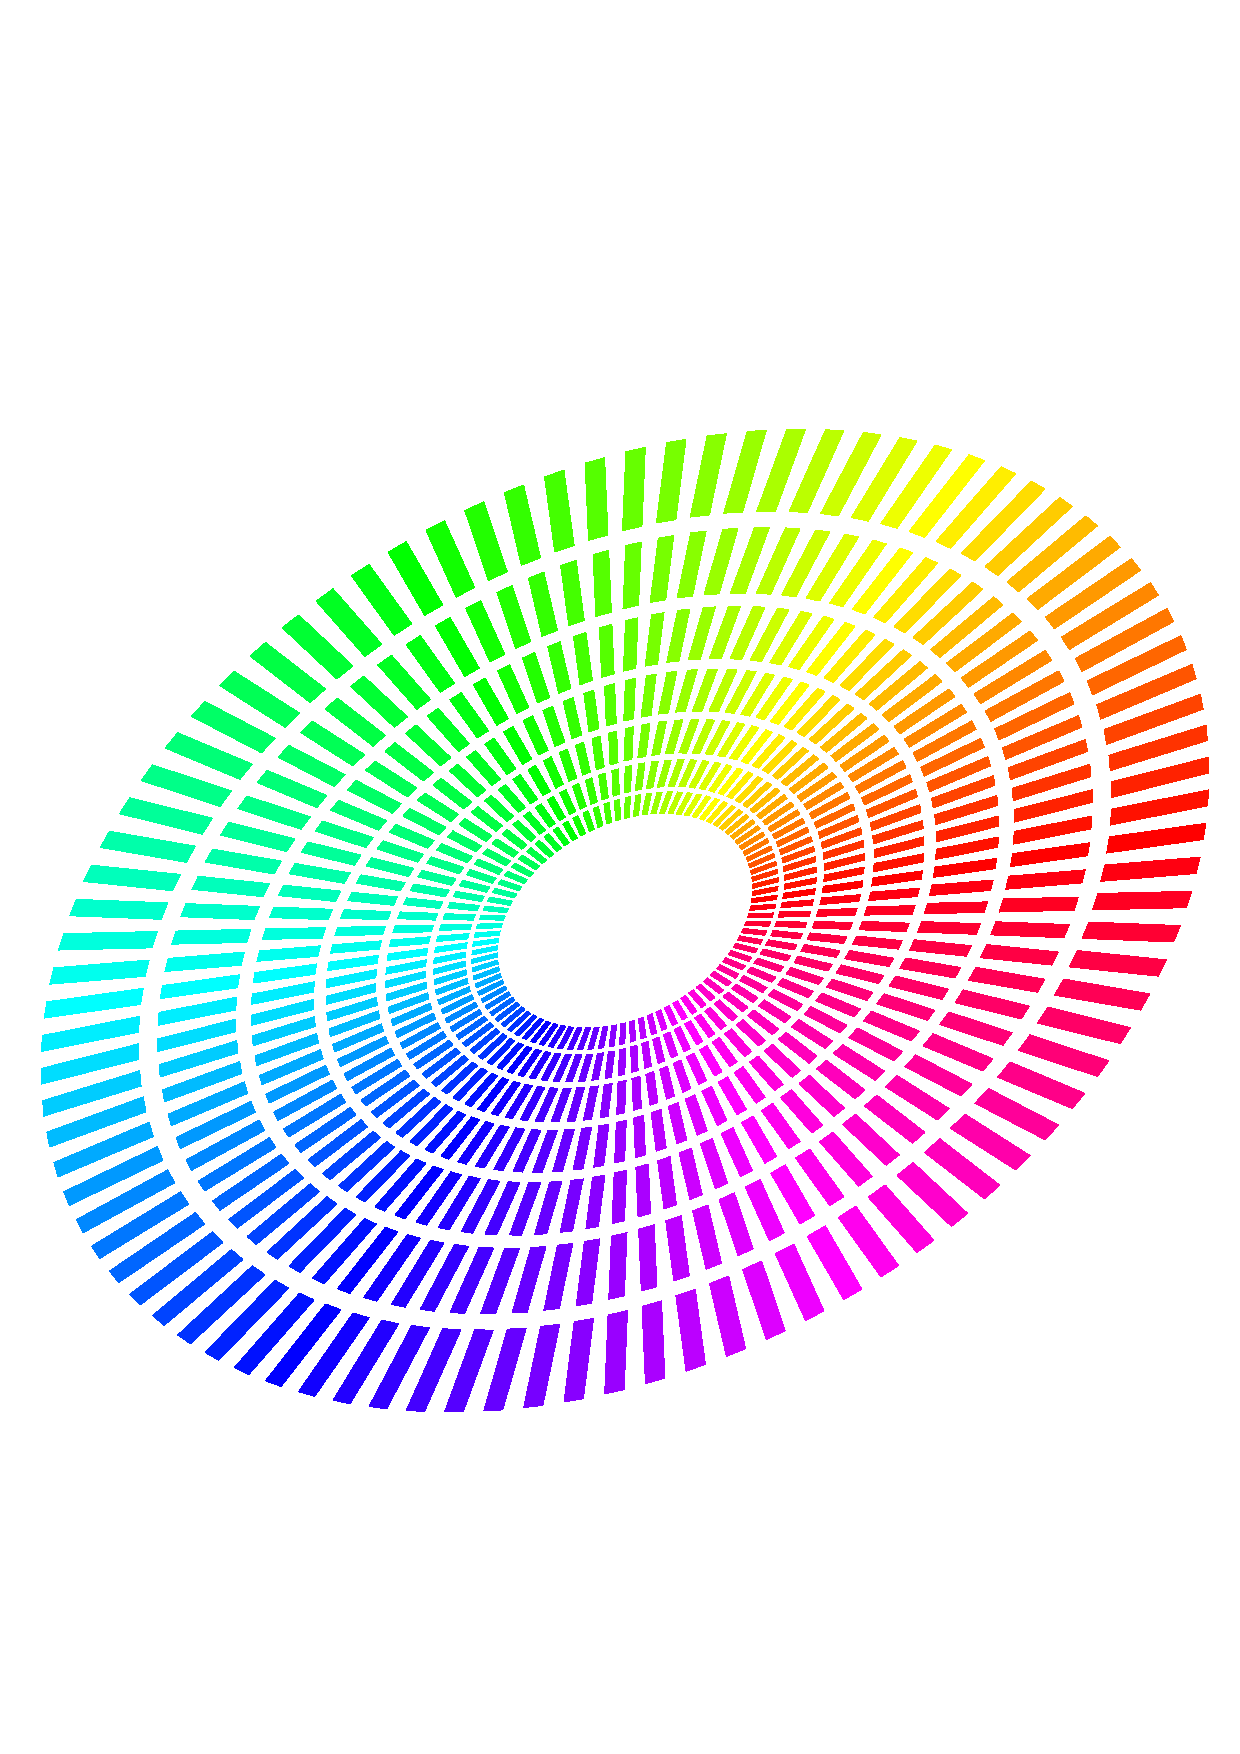
\includegraphics[width=8cm]{figure}
  \caption{A colourful picture.}
  \label{Figure:figex}
\end{figure}

This page shows you a subfigure example in \fref{Figure:figsubex}.
\begin{figure}[!htb]
  \centering
  \subfigure[The left caption]{
    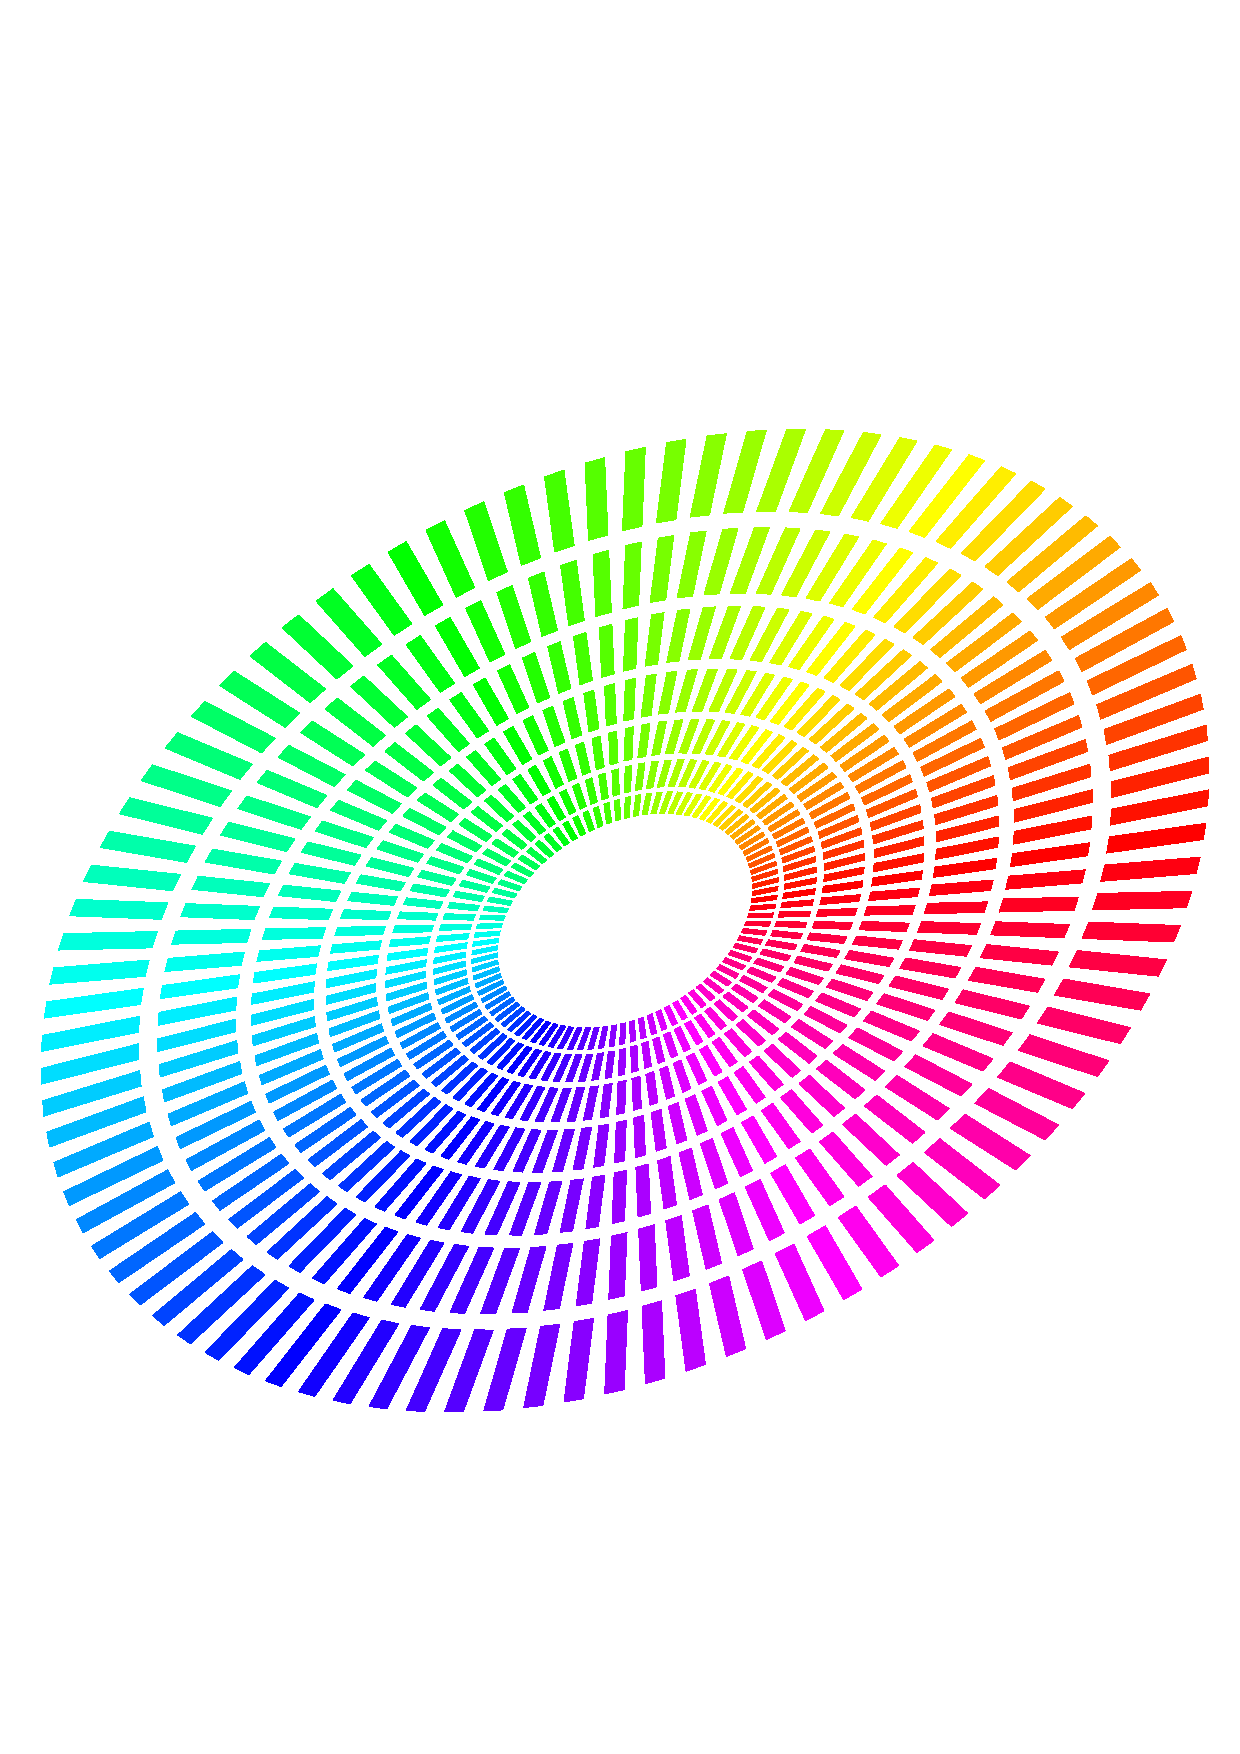
\includegraphics[width=4.2cm]{figure}
    \label{Figure:figsubex:left}
  }
  \subfigure[The right caption]{
    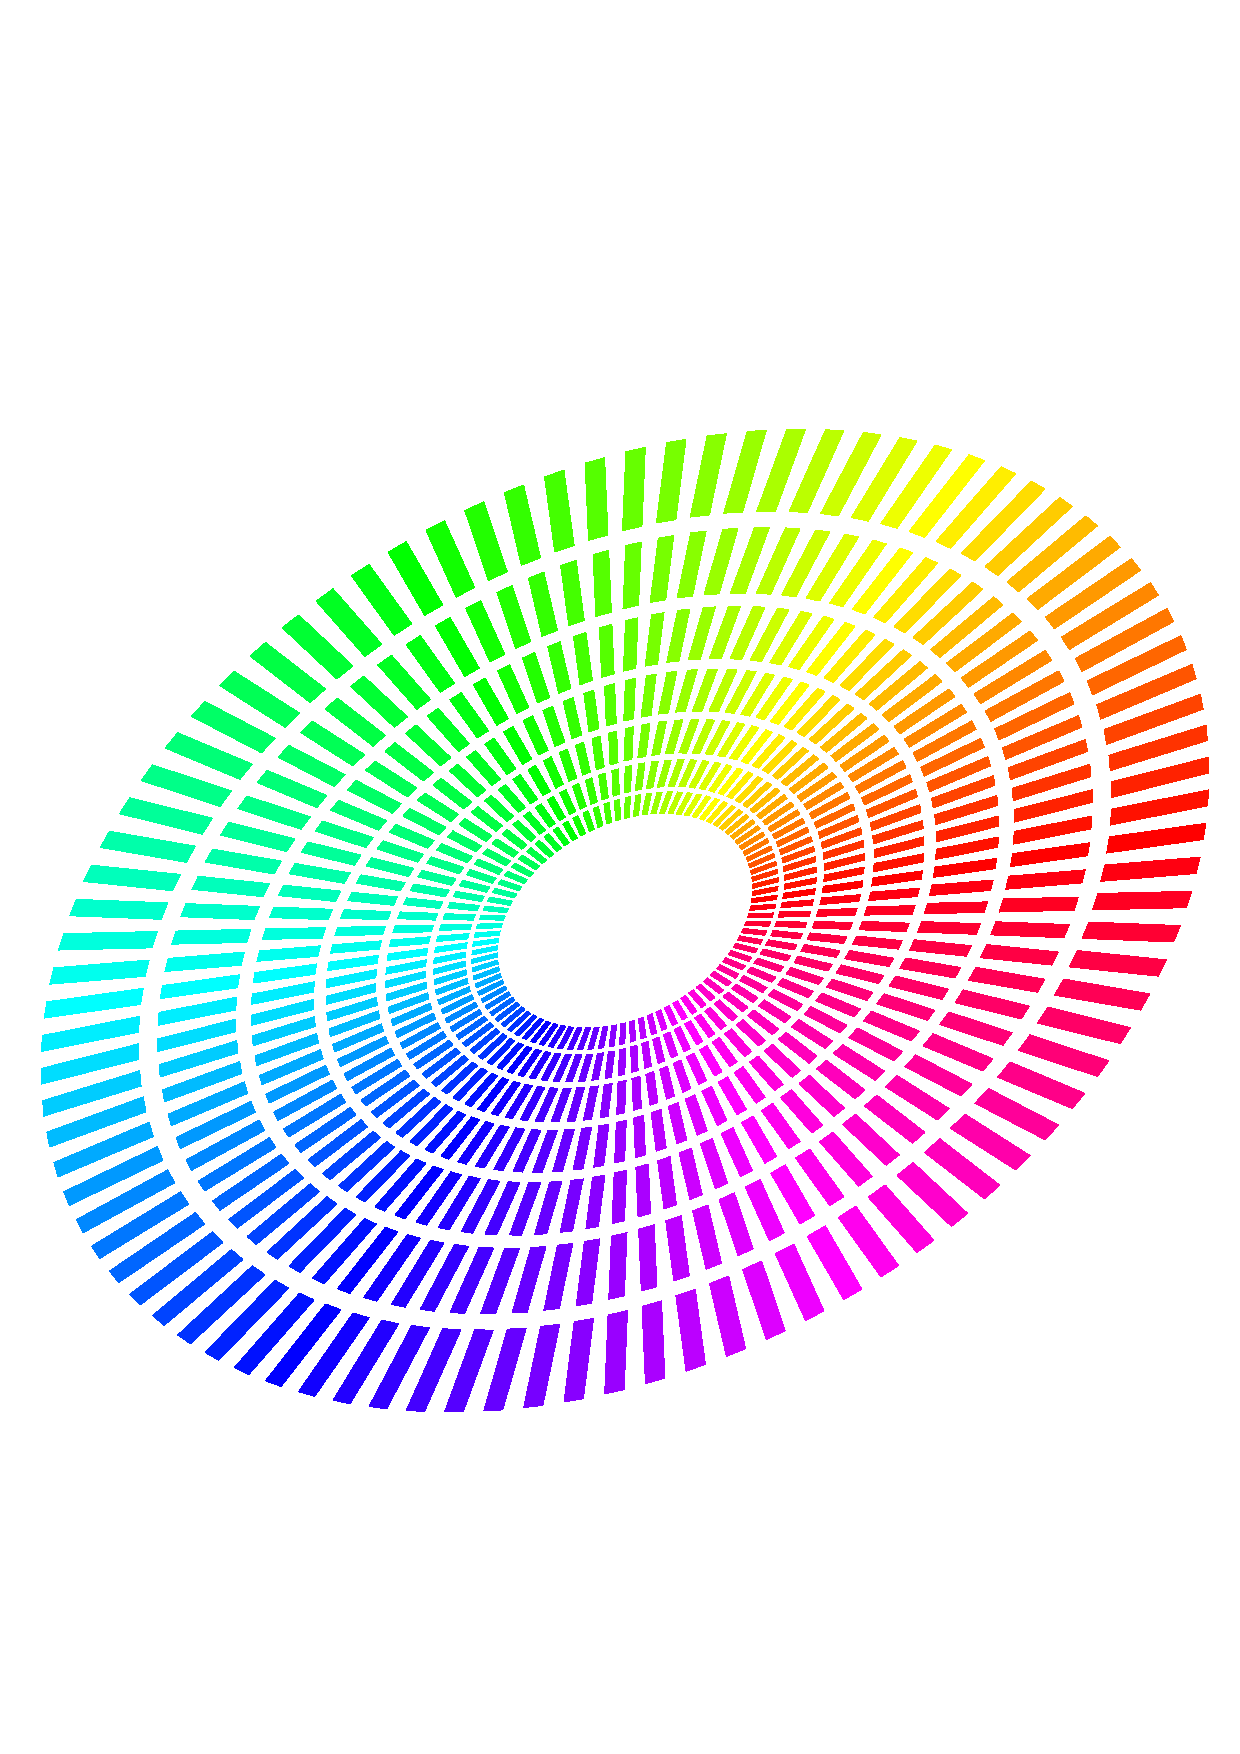
\includegraphics[width=4.2cm]{figure}
    \label{Figure:figsubex:right}
  }
  \caption{A doubly colourful picture.}
  \label{Figure:figsubex}
\end{figure}

%% ----------------------------------------------------------------
%% Conclusions.tex
%% ---------------------------------------------------------------- 
\chapter{Conclusions} \label{Chapter: Conclusions}
It works.

\begin{lstlisting}[caption=Listing of what an example listing would be like]
This is a test listing

The test listing has several lines
to show how the listings
will be displayed
\end{lstlisting}
\appendix
%% ----------------------------------------------------------------
%% AppendixA.tex
%% ---------------------------------------------------------------- 
\chapter{Stuff} \label{Chapter:Stuff}
The following gets in the way of the text....

\backmatter
%<*testthesis|testminithesis|testprogress>
\chapter{Glossary [if relevant]}
%</testthesis|testminithesis|testprogress>
\bibliographystyle{plainnat}
\bibliography{UOS}
%<*testthesis|testminithesis|testprogress>
\chapter{Bibliography}
To use bibliography as well as the references section use the \texttt{multibbl} package.
\chapter{Index [if relevant]}
%</testthesis|testminithesis|testprogress>
%</testthesis|testminithesis|testprogress|testproject|testreport|testgdp>
%<*testgdpsummary>
\section*{Introduction}
\section*{Objectives}
\section*{Resources}
\section*{Constraints}
\section*{Approaching the task}
\section*{Team Organisation}
\section*{Important Results}
\section*{Conclusions}
\section*{Recommendations}
%</testgdpsummary>
%<*introduction>
\chapter{Introduction} \label{Chapter:Introduction}
%</introduction>
%<*testarticle>
\section{Introduction} \label{Section:Introduction}
%</testarticle>
%<*introduction|testarticle>
You probably found all the files from \cite{Longman:2019:templ},
they were originally made from \cite{Gunn:2001:pdflatex}.
Template specific instructions can be found at:
\url{https://git.soton.ac.uk/el7g15/uos-latex-template-instructions}.

\tref{Table:tabex} illustrates the results of some arbitrary example work.
\begin{table}[!htb]
  \centering
  \begin{tabular}{cc}
  \toprule
  \textbf{Training Error} & \textbf{Testing Error}\\
  \midrule
  0 & $\infty$\\
  \bottomrule
  \end{tabular}
  \caption{The Results}
  \label{Table:tabex}
\end{table}

\fref{Figure:figex} shows why this is the case.
\begin{figure}[!htb]
  \centering
  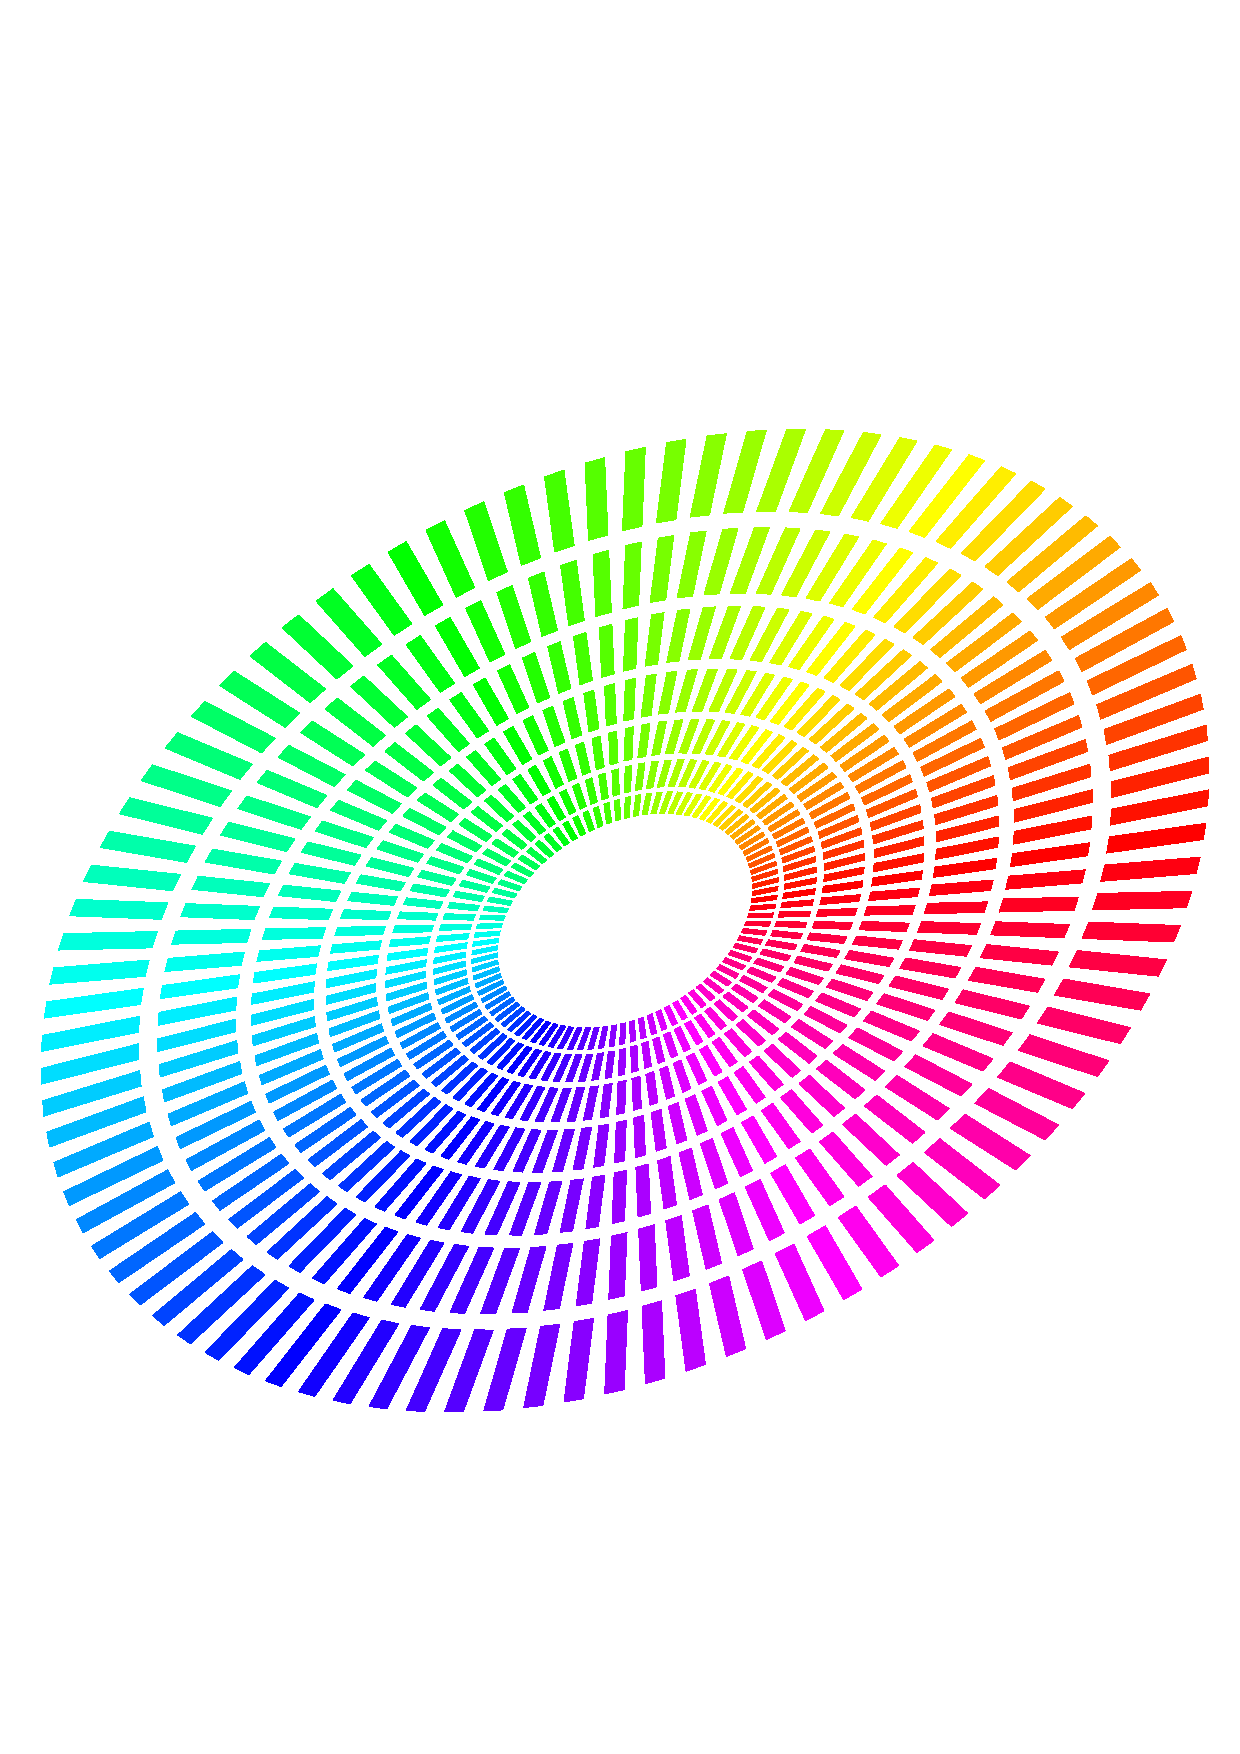
\includegraphics[width=8cm]{figure}
  \caption{A colourful picture.}
  \label{Figure:figex}
\end{figure}

This page shows you a subfigure example in \fref{Figure:figsubex}.
\begin{figure}[!htb]
  \centering
  \subcaptionbox{The left caption}{
    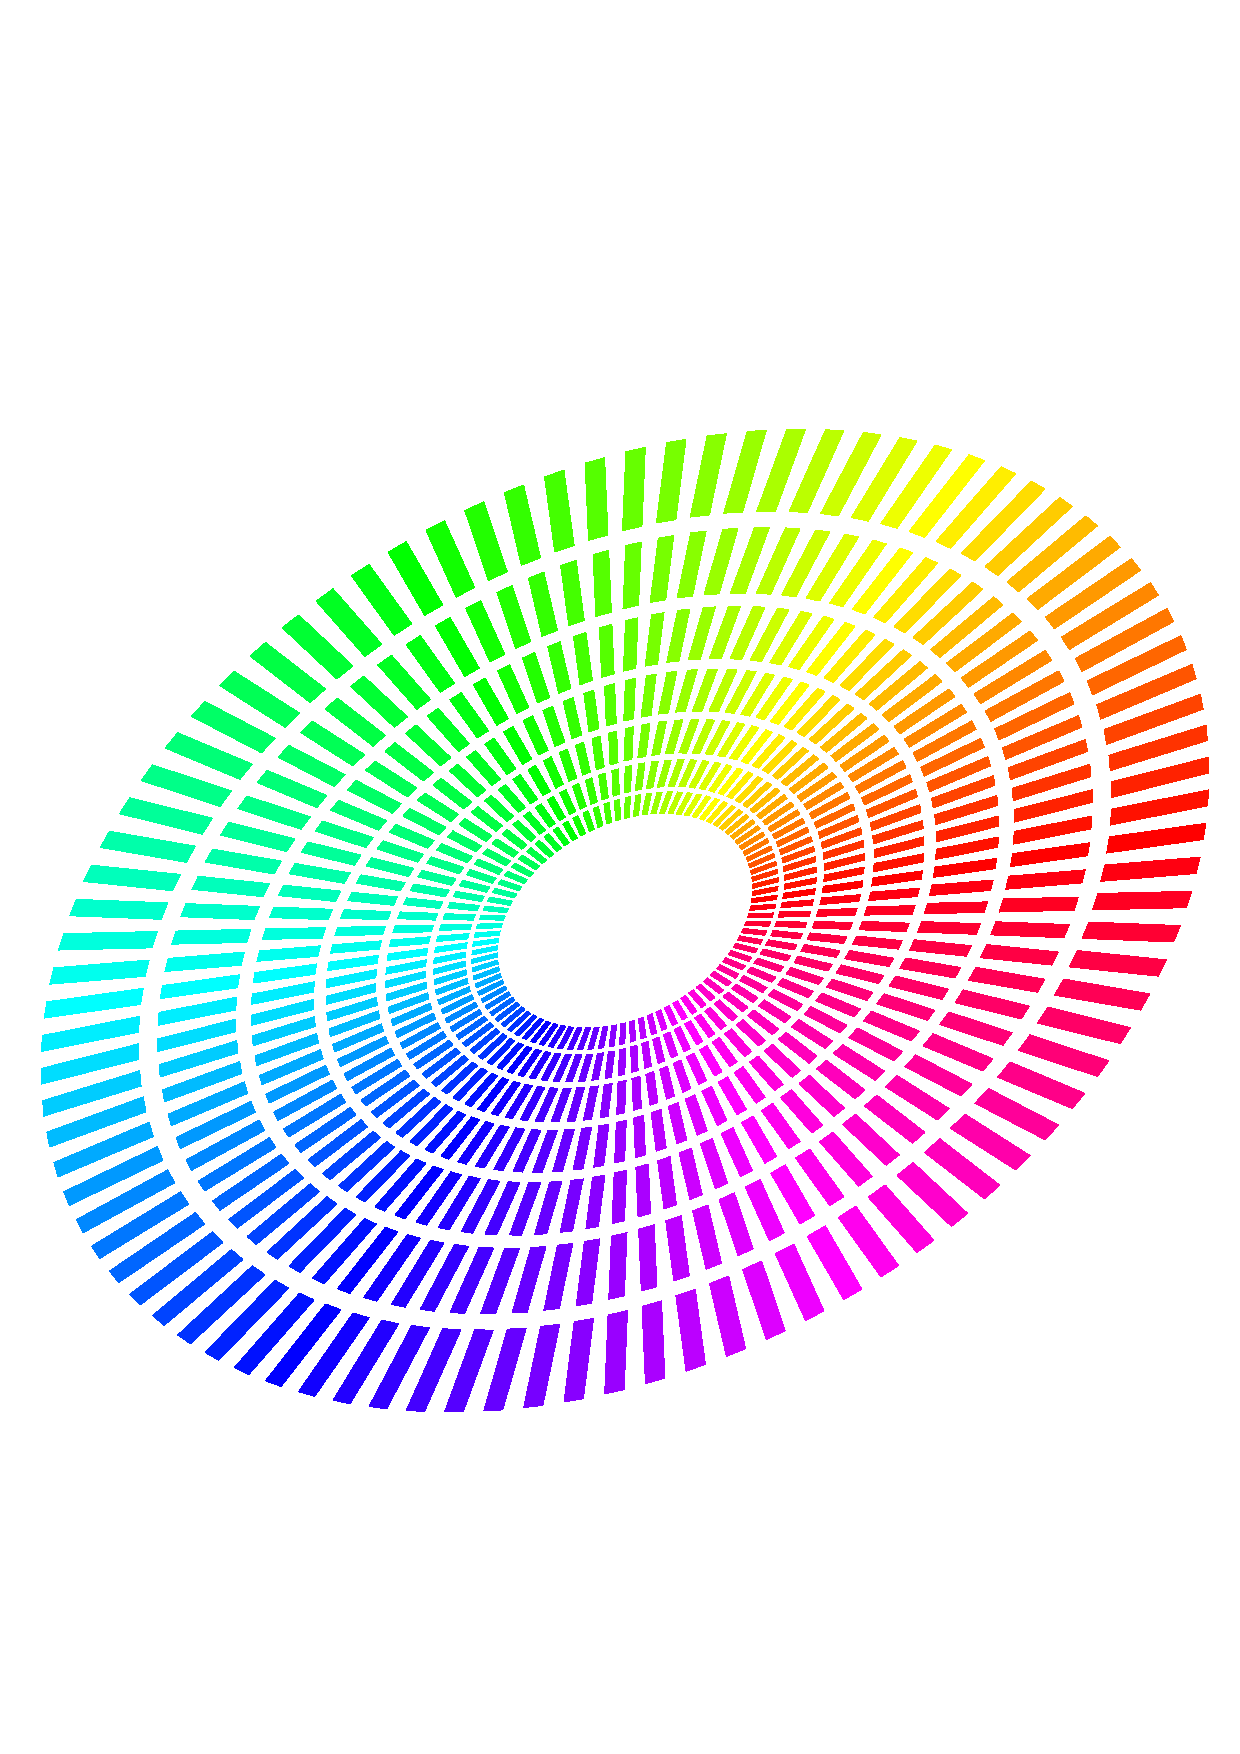
\includegraphics[width=4.2cm]{figure}
    \label{Figure:figsubex:left}
  }
  \subcaptionbox{The right caption}{
    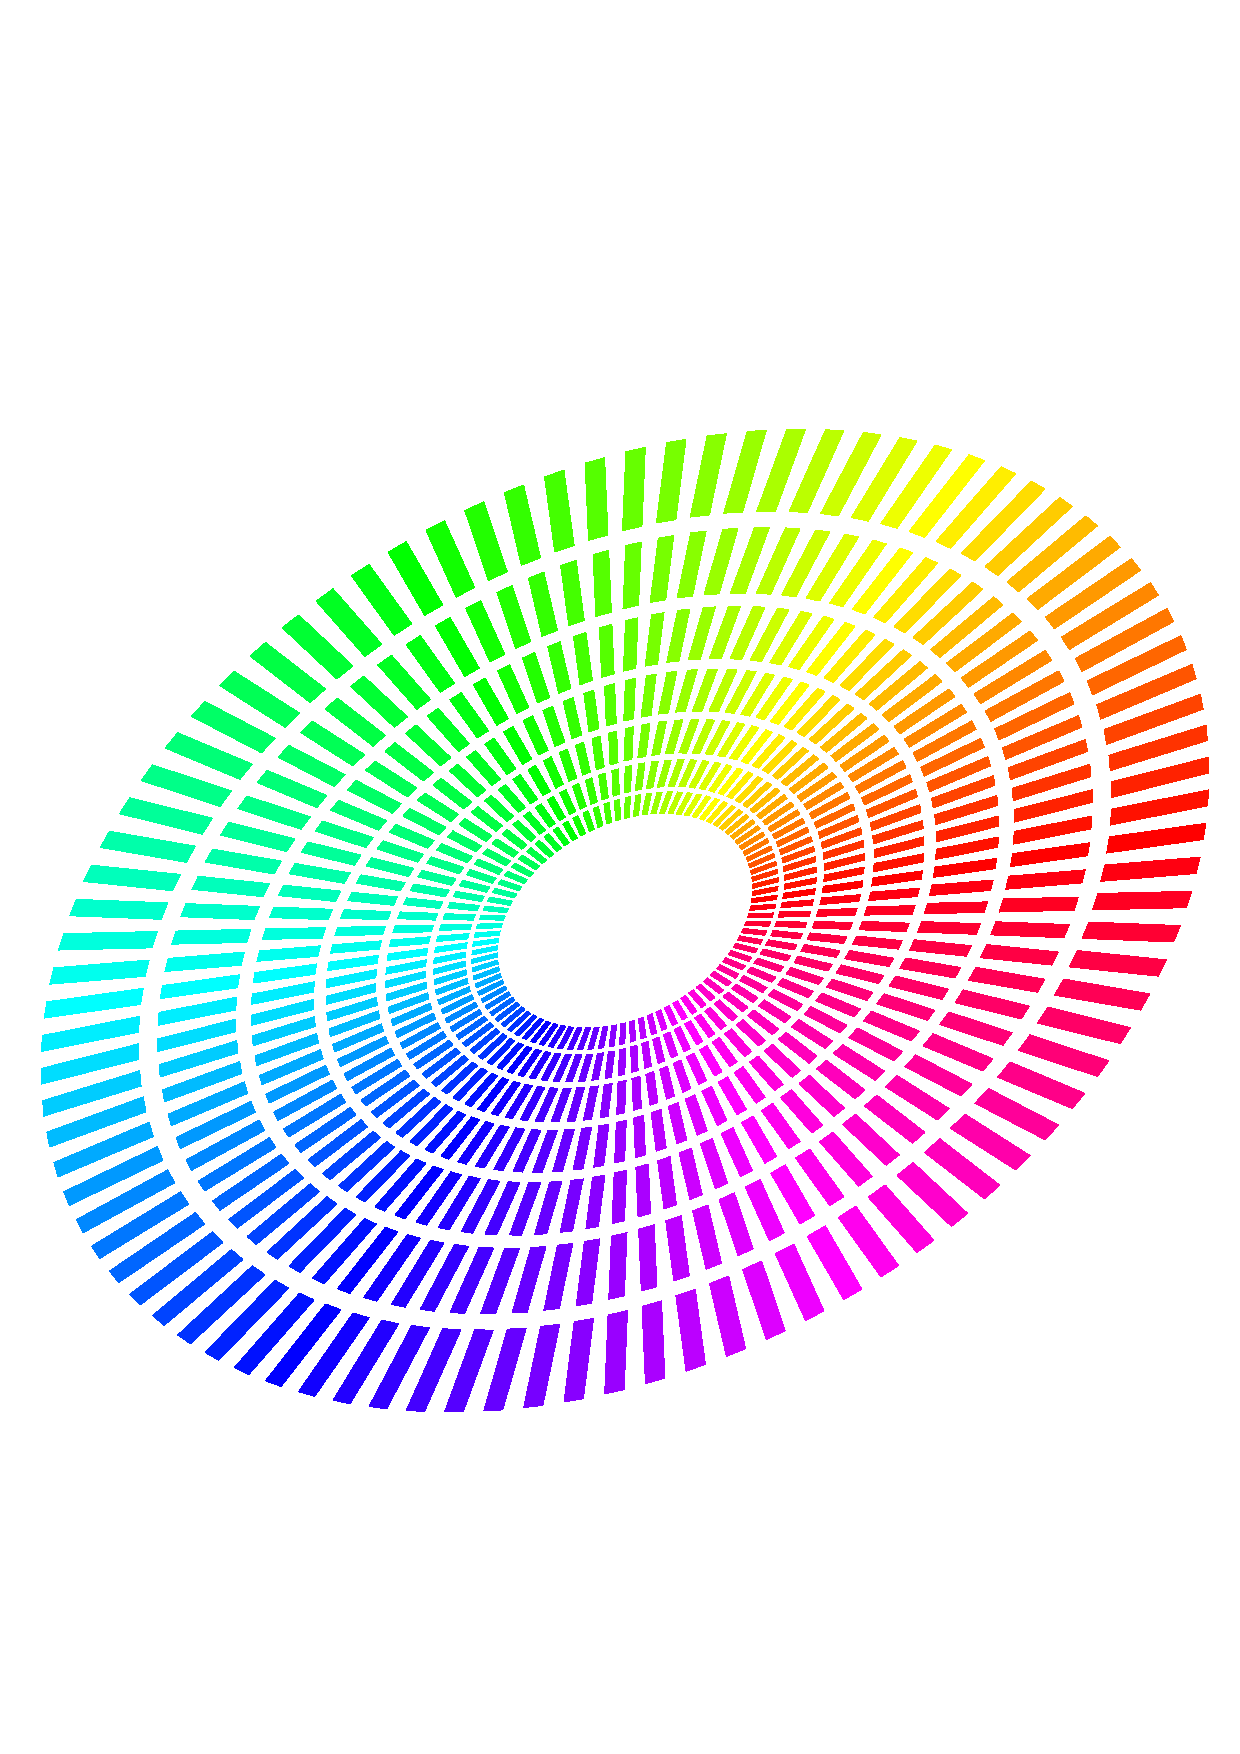
\includegraphics[width=4.2cm]{figure}
    \label{Figure:figsubex:right}
  }
  \caption{A doubly colourful picture.}
  \label{Figure:figsubex}
\end{figure}
Lorem ipsum dolor sit amet, consectetur adipiscing elit. Donec rutrum sodales ligula, ac aliquam sem interdum at. Ut commodo pulvinar ipsum. Aliquam et diam sed nibh tincidunt mollis vitae quis nunc. In vel ante vitae felis semper malesuada sed a metus. Aliquam semper metus vel metus imperdiet, quis mollis nisi volutpat. Integer in convallis erat, et auctor dui. Phasellus id tristique tortor. Mauris ac nisi ut mi pulvinar interdum. Donec quis nibh tempus erat lobortis dapibus non a nunc. Nulla laoreet tempus fringilla. Aliquam pulvinar, sapien eu interdum gravida, libero urna dapibus sem, sodales efficitur lorem nunc et justo. Proin vitae dolor nisl.

\section{A Section of a chapter}
Nulla molestie velit sed dui ullamcorper viverra. Fusce placerat vulputate lacus eu consequat. Cras ullamcorper vel mauris quis aliquam. Curabitur non varius elit, eget commodo urna. Phasellus erat libero, faucibus elementum augue eget, malesuada fringilla purus. Quisque pulvinar, lectus sit amet ultricies tristique, eros nunc commodo lacus, nec ultrices risus lorem vitae diam. Cras ac ornare nisi.

\subsection{Some quotes}

Nam egestas felis euismod erat tincidunt ornare. Nulla hendrerit tempor purus ac consequat. Aliquam commodo, ipsum vestibulum lobortis semper, urna turpis sagittis dolor, id ullamcorper nulla nisl vitae ex. Vivamus ut metus vel velit rhoncus pulvinar sit amet nec diam. Aliquam aliquet, enim eget efficitur euismod, velit arcu mattis nisl, a mollis dui leo vel libero. Nullam porttitor convallis magna ut feugiat. `Cras at ultrices metus.' Nullam vulputate quis justo sit amet pharetra. Praesent sodales eros non suscipit gravida.
\begin{quote}
Lorem ipsum dolor sit amet, consectetur adipiscing elit. Donec rutrum sodales ligula, ac aliquam sem interdum at.
\end{quote}

Pellentesque sodales lobortis feugiat. Vivamus volutpat mauris id odio aliquam maximus sed sit amet nibh. Fusce odio tortor, aliquam et mauris facilisis, interdum placerat tortor. Suspendisse dapibus, massa eget cursus congue, mi lectus luctus nisl, vitae sagittis ligula ante sit amet enim. Donec quis sapien vel ex vestibulum porta. Vivamus mattis sodales turpis, id interdum justo ullamcorper a. Aenean ornare urna turpis, id fermentum eros commodo aliquet. Class aptent taciti sociosqu ad litora torquent per conubia nostra, per inceptos himenaeos. Donec cursus pretium ex at mollis. Vestibulum ante ipsum primis in faucibus orci luctus et ultrices posuere cubilia Curae; Sed at diam quam. Etiam a sollicitudin dui. Nulla facilisi. Phasellus condimentum tincidunt ipsum. Sed dignissim neque a porttitor finibus. Maecenas pretium dictum lorem vitae viverra.
\begin{quote}
The \verb|\attrib| macro attributes block elements, for example when citing
a reference after a block quotation.
\ifdefined\attrib\attrib{\cite{attribpackage}}\fi
\end{quote}

Donec vitae massa nisi. Praesent sed sollicitudin urna. Suspendisse vitae cursus tortor. In egestas quis dolor ac porttitor. Pellentesque suscipit leo nisi, a semper nunc interdum quis. Aenean massa magna, aliquam imperdiet lorem vitae, vestibulum dignissim nunc. Nunc molestie eleifend dui et porta. Sed auctor eu nunc vel faucibus. Integer et finibus metus, pharetra egestas velit. Sed nec magna semper, rutrum diam vitae, accumsan sapien. Donec congue viverra luctus.
%</introduction|testarticle>
%<*conclusions>
\chapter{Conclusions} \label{Chapter: Conclusions}
%</conclusions>
%<*testarticle>
%% ----------------------------------------------------------------
\section{Conclusions} \label{Section: Conclusions}
%</testarticle>
%<*conclusions|testarticle>
It works.
%</conclusions|testarticle>
%<*testarticle>
\acknowledgements{Thanks to no one.}
\backmatter
\appendix
\bibliographystyle{plainnat}
\bibliography{UOS}
%</testarticle>
%<*appendix|testarticle>
%<*appendix>
\chapter{Stuff} \label{Chapter:Stuff}
%</appendix>
%<*testarticle>
%% ----------------------------------------------------------------
\section{Stuff} \label{Section:Stuff}
%</testarticle>
The following gets in the way of the text....
%</appendix|testarticle>
%<*testthesis|testminithesis|testprogress|testproject|testreport|testarticle|testgdp|testgdpsummary>
\end{document}
%% ----------------------------------------------------------------
%</testthesis|testminithesis|testprogress|testproject|testreport|testarticle|testgdp|testgdpsummary>
%    \end{macrocode}
%
% \subsection{Example Figure}
%
%    \begin{macrocode}
%<*figure>
%%BoundingBox: 0 150 600 650
%%EndComments
0.0 setlinewidth
/length 0.1 def
/width 0.02 def
/hsvcircle {
gsave
    /h 0.0 def
    0 4 360 {
    pop
    gsave
    0.5 0.0 translate
    newpath
    0.0 0.0 moveto
    length 0.0 lineto
    length width lineto
    0.0 width lineto
    closepath
    h 1.0 1.0 sethsbcolor
    fill
    grestore
    /h h 4 360 div add def
    4 rotate
    } for
grestore
} def
0.0 setlinewidth
0.0 setgray
300 400 translate
500 500 scale
30 rotate
1.0 0.7 scale
-30 rotate
hsvcircle
0.8 0.8 scale
hsvcircle
0.8 0.8 scale
hsvcircle
0.8 0.8 scale
hsvcircle
0.8 0.8 scale
hsvcircle
0.8 0.8 scale
hsvcircle
0.8 0.8 scale
hsvcircle
showpage
%</figure>
%    \end{macrocode}
%
% \subsection{Definitions File}
%
%    \begin{macrocode}
%<*definitions>
\newcommand{\BibTeX}{{\rm B\kern-.05em{\sc i\kern-.025em b}\kern-.08em T\kern-.1667em\lower.7ex\hbox{E}\kern-.125emX}}

%% People
\newcounter{address}
\setcounter{address}{1}
\renewcommand{\theaddress}{\textsuperscript{\fnsymbol{address}}}
\newcommand{\address}[1]{\refstepcounter{address}\theaddress#1\\}
\newcommand{\Name}[3]{\texorpdfstring{\href{mailto:#3}{#2}#1}{#2}\xspace}
\newcommand{\SteveRGunn}[1]{\Name{#1}{Steve R. Gunn}{S.R.Gunn@ecs.soton.ac.uk}}

%% Dingbats
\newcommand{\tick}{\ding{51}}
\newcommand{\cross}{\ding{55}}

%% Calculus
\newcommand{\pd}[2]{\ensuremath{\frac{\partial #1}{\partial #2}}\xspace}
\newcommand{\fd}[2]{\ensuremath{\frac{d #1}{d #2}}\xspace}
\newcommand{\dint}{\ensuremath{\int\!\!\!\int}\xspace}
\newcommand{\tint}{\ensuremath{\int\!\!\!\int\!\!\!\int}\xspace}

%% Math Sets
\newcommand{\Q}[1]{\ensuremath{\mathbb{#1}}\xspace}
\newcommand{\R}{\Q{R}}

%% Matrix, Vector
\newcommand{\V}[1]{\ensuremath{\boldsymbol{#1}}\xspace}
\newcommand{\M}[1]{\ensuremath{\boldsymbol{#1}}\xspace}
\newcommand{\0}{\V{0}}
\newcommand{\1}{\V{1}}
\newcommand{\I}{\M{I}}

%% Math Functions
\newcommand{\F}[1]{\ensuremath{\mathrm{#1}}\xspace}
\newcommand{\sgn}{\F{sgn}}
\newcommand{\tr}{\F{trace}}
\newcommand{\diag}{\F{diag}}

%% Math Names
\newcommand{\N}[1]{\ensuremath{\mathit{#1}}\xspace}

%% Data
\newcommand{\mc}[1]{\ensuremath{\mathcal{#1}}\xspace}
\newcommand{\Hyp}{\mc{H}}
\newcommand{\D}{\mc{D}}

%% Kernel
\newcommand{\K}{\M{K}}
\newcommand{\eins}{\texorpdfstring{\ensuremath{\epsilon}}{\textepsilon}-insensitive\xspace}
\newcommand{\e}{\ensuremath{\epsilon}\xspace}
\newcommand{\Bxi}{\ensuremath{\boldsymbol{\xi}}\xspace}
\newcommand{\Kanova}{\ensuremath{\mathit{K_{ANOVA}}}\xspace}
\newcommand{\Kspline}{\ensuremath{\mathit{K_{spline}}}\xspace}

%% Bayesian
\newcommand{\MP}{\ensuremath{\mathit{{\scriptscriptstyle \hspace{-1.5pt}M\hspace{-1.5pt}P}}}\xspace}
\newcommand{\ML}{\ensuremath{\mathit{{\scriptscriptstyle \hspace{-1.5pt}M\hspace{-1.5pt}L}}}\xspace}
\newcommand{\Qw}{\ensuremath{Q_{\w}(\w)}\xspace}
\newcommand{\Qa}{\ensuremath{Q_{\Ba}(\Ba)}\xspace}
\newcommand{\Qb}{\ensuremath{Q_{\beta}(\beta)}\xspace}
\newcommand{\wMPab}{\ensuremath{\w_{\MP|\bar {\Ba},\bar \beta}}\xspace}
\newcommand{\wMP}{\ensuremath{\w_{\MP}}\xspace}
\newcommand{\yMP}{\ensuremath{y_{\MP}}\xspace}
\newcommand{\BaMP}{\ensuremath{\Ba_{\hspace{1pt}\MP}}\xspace}
\newcommand{\aMP}{\ensuremath{\alpha_{\hspace{1pt}\MP}}\xspace}
\newcommand{\bMP}{\ensuremath{\beta_{\hspace{1pt}\MP}}\xspace}
\newcommand{\Sab}{\ensuremath{\M{\Sigma}_{\bar \Ba,\bar \beta}}\xspace}
\newcommand{\Ba}{\ensuremath{\boldsymbol{\alpha}}\xspace}
\newcommand{\Bb}{\ensuremath{\boldsymbol{\beta}}\xspace}
\newcommand{\Bm}{\ensuremath{\boldsymbol{\mu}}\xspace}
\newcommand{\BL}{\ensuremath{\boldsymbol{\Lambda}}\xspace}
\newcommand{\BPhi}{\ensuremath{\boldsymbol{\Phi}}\xspace}
\newcommand{\SMP}{\ensuremath{\M{\Sigma}_{\MP}}\xspace}

\newcommand{\Pa}{\ensuremath{P(\alpha|\mathcal{H})}\xspace}
\newcommand{\Pb}{\ensuremath{P(\beta|\mathcal{H})}\xspace}
\newcommand{\Pab}{\ensuremath{P(\alpha,\beta|\mathcal{H})}\xspace}
\newcommand{\Pw}{\ensuremath{P(\w|\mathcal{H})}\xspace}
\newcommand{\PD}{\ensuremath{P(\D|\mathcal{H})}\xspace}
\newcommand{\PwIa}{\ensuremath{P(\w|\alpha,\mathcal{H})}\xspace}
\newcommand{\PDIwb}{\ensuremath{P(\D|\w,\beta,\mathcal{H})}\xspace}
\newcommand{\PDwab}{\ensuremath{P(\D,\w,\alpha,\beta|\mathcal{H})}\xspace}
\newcommand{\PDIw}{\ensuremath{P(\D|\w,\mathcal{H})}\xspace}
\newcommand{\PwID}{\ensuremath{P(\w|\D,\mathcal{H})}\xspace}
\newcommand{\PwabID}{\ensuremath{P(\w,\alpha,\beta|\D,\mathcal{H})}\xspace}

\newcommand{\PanH}{\ensuremath{P(\alpha)}\xspace}
\newcommand{\PbnH}{\ensuremath{P(\beta)}\xspace}
\newcommand{\PabnH}{\ensuremath{P(\alpha,\beta)}\xspace}
\newcommand{\PwnH}{\ensuremath{P(\w)}\xspace}
\newcommand{\PDnH}{\ensuremath{P(\D)}\xspace}
\newcommand{\PwIanH}{\ensuremath{P(\w|\alpha)}\xspace}
\newcommand{\PDIwbnH}{\ensuremath{P(\D|\w,\beta)}\xspace}
\newcommand{\PDwabnH}{\ensuremath{P(\D,\w,\Ba,\beta)}\xspace}
\newcommand{\PDIwnH}{\ensuremath{P(\D|\w)}\xspace}
\newcommand{\PwIDnH}{\ensuremath{P(\w|\D)}\xspace}
\newcommand{\PwabIDnH}{\ensuremath{P(\w,\alpha,\beta|\D)}\xspace}

\newcommand{\PDwBab}{\ensuremath{P(\D,\w,\Ba,\beta|\mathcal{H})}\xspace}
\newcommand{\PwIBa}{\ensuremath{P(\w|\Ba,\mathcal{H})}\xspace}
\newcommand{\PBab}{\ensuremath{P(\Ba,\beta|\mathcal{H})}\xspace}
\newcommand{\PwBabID}{\ensuremath{P(\w,\Ba,\beta|\D,\mathcal{H})}\xspace}

\newcommand{\PBanH}{\ensuremath{P(\Ba)}\xspace}
\newcommand{\PwIBanH}{\ensuremath{P(\w|\Ba)}\xspace}

%% Snakes
\newcommand{\Esnake}{\ensuremath{\mathit{E_{snake}}}\xspace}
\newcommand{\Eimage}{\ensuremath{\mathit{E_{image}}}\xspace}
\newcommand{\Econt}{\ensuremath{\mathit{E_{cont}}}\xspace}
\newcommand{\Ecurv}{\ensuremath{\mathit{E_{curv}}}\xspace}
\newcommand{\Eint}{\ensuremath{\mathit{E_{int}}}\xspace}
\newcommand{\Eext}{\ensuremath{\mathit{E_{ext}}}\xspace}
\newcommand{\Eterm}{\ensuremath{\mathit{E_{term}}}\xspace}
\newcommand{\Eline}{\ensuremath{\mathit{E_{line}}}\xspace}
\newcommand{\Eedge}{\ensuremath{\mathit{E_{edge}}}\xspace}
\newcommand{\Econ}{\ensuremath{\mathit{E_{con}}}\xspace}
\newcommand{\Eangle}{\ensuremath{\mathit{E_{angle}}}\xspace}
\newcommand{\Elshape}{\ensuremath{\mathit{E_{lshape}}}\xspace}
\newcommand{\Eedgedir}{\ensuremath{\mathit{E_{edgedir}}}\xspace}
\newcommand{\Emodel}{\ensuremath{\mathit{E_{model}}}\xspace}
\newcommand{\wte}{\ensuremath{\mathit{w_{term}}}\xspace}
\newcommand{\wli}{\ensuremath{\mathit{w_{line}}}\xspace}
\newcommand{\wed}{\ensuremath{\mathit{w_{edge}}}\xspace}
\newcommand{\wco}{\ensuremath{\mathit{w_{con}}}\xspace}


%% Environments
\newcounter{alg}
\newenvironment{algorithm}[1]
{
    \stepcounter{alg}
    \begin{table}[htb]
    \centering
    \begin{tabular}[t]{ll}
    \hline&\\
    \multicolumn{2}{l}{\bf Algorithm \arabic{alg}: #1}\\&\\
} {
    &\\
    \hline
    \end{tabular}
    \end{table}
}
%</definitions>
%    \end{macrocode}
%
% \subsection{References File}\label{references}
%
%    \begin{macrocode}
%<*references>
@MISC{Longman:2019:templ,
  author =       {E. Longman},
  title =        {{University of Southampton LaTeX documents}},
  year =         {2019},
  NOTE =     "\url{https://library.soton.ac.uk/thesis/templates} and
             \url{https://git.soton.ac.uk/el7g15/uos-latex-template}",
}
@MISC{Gunn:2001:pdflatex,
  author =       {S.R. Gunn},
  title =        {PDFLaTeX Instructions},
  year =         {2001},
  url =          {http://www.ecs.soton.ac.uk/~srg/softwaretools/document/}
}
@MISC{Lovell:2011:updated,
  author =       {C. J. Lovell},
  title =        {Updated templates},
  year =         {2011}
}
@MISC{Gunn:2011:updated2,
  author =       {S.R. Gunn and C. J. Lovell},
  title =        {Updated templates reference 2},
  year =         {2011}
}
@MISC{attribpackage,
  author =       {Matt Swift},
  title =        {The attrib LaTeX package
attribution of block elements (Frankenstein’s hat)},
  year =         {1999},
  url =          {http://cs.brown.edu/about/system/managed/latex/doc/attrib.pdf}
}

%</references>
%    \end{macrocode}
%
% \subsection{Bibliography Style File}
%    This has now been changed to the ordinary plainnat as natbib caught up
%
% \Finale
%
\endinput
